\cotefile{145}
\scanpage{1}
\figure{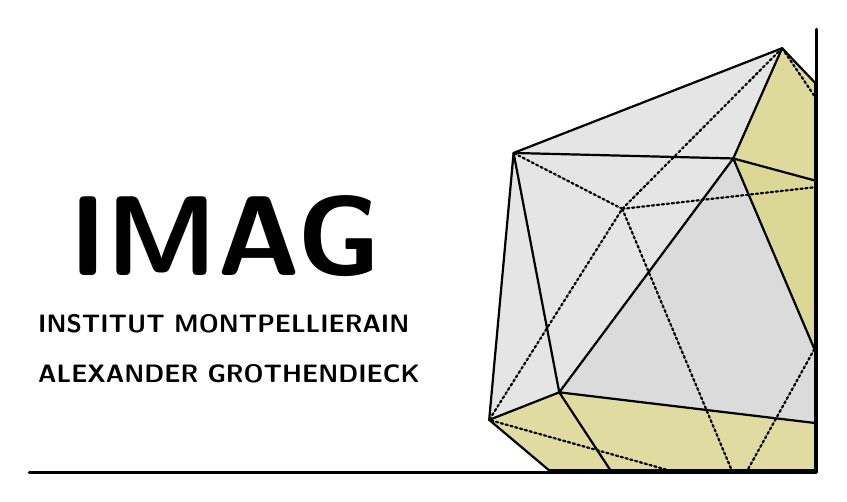
\begin{tikzpicture}[x=1cm,y=1cm,line cap=round,line join=round]
\node[anchor=west,font=\sffamily\bfseries,scale=4.1] at (0,3.0) {IMAG};
\node[anchor=west,font=\sffamily\bfseries,scale=0.91] at (0,1.88) {INSTITUT MONTPELLIERAIN};
\node[anchor=west,font=\sffamily\bfseries,scale=0.91] at (0,1.25) {ALEXANDER GROTHENDIECK};
\begin{scope}
\clip (5.65,0) rectangle (10.0,5.45);
\coordinate (A) at (6.15,4.05); \coordinate (B) at (9.56,5.38);
\coordinate (C) at (10.32,4.60); \coordinate (D) at (8.94,3.98);
\coordinate (E) at (5.84,0.66); \coordinate (F) at (6.73,1.01);
\coordinate (G) at (9.98,0.62); \coordinate (H) at (10.20,3.64);
\coordinate (I) at (7.53,3.34); \coordinate (J) at (6.60,0.02);
\coordinate (K) at (9.97,1.56);
\fill[gray!20] (A)--(B)--(D)--(F)--(E)--cycle;
\fill[gray!28] (D)--(F)--(G)--(K)--cycle;
\fill[olive!30] (B)--(C)--(H)--(D)--cycle;
\fill[olive!32] (D)--(H)--(K)--cycle;
\fill[olive!28] (E)--(F)--(G)--(9.98,0.02)--(J)--cycle;
\draw[thick] (B)--(A)--(E)--(J)--(9.98,0.02)--(9.98,4.94)--(B)--(D)--(A);
\draw[thick] (D)--(H) (D)--(K) (D)--(F)--(A) (E)--(F)--(G) (F)--(7.38,0.02);
\draw[thick,densely dotted] (B)--(I)--(E)--(8.12,0.02) (I)--(A) (I)--(H) (I)--(8.92,0.02) (K)--(9.12,0.02) (B)--(9.98,4.76);
\end{scope}
\draw[line width=1.2pt] (0,-0.01)--(10.0,-0.01)--(10.0,5.62);
\end{tikzpicture}} % crop-candidate: scan 1

\scanpage{2}
\deleted{bien \unsure{distinguer} $\bar D_{J,\alpha}$ de $\bar D_J$, \unsure{cf. 9}}
\deleted{\diagram{\begin{tikzcd}
\bar U_{J',\alpha'} \arrow[r] \arrow[d] & \bar U_{J,\alpha} \arrow[r] \arrow[d] & \bar U \arrow[d] \\
U_{J',\alpha'} \arrow[r] & U_{J,\alpha} \arrow[r] & U
\end{tikzcd}}}

\diagram{\begin{tikzcd}[column sep=small]
D=U(\mathbb C)^{\sim} \arrow[rr] \arrow[dr,"\pi"'] && \widetilde U(\mathbb C)\deleted{\unsure{\ne U}} \arrow[dl,"\hat\pi"] \\
& U(\mathbb C) &
\end{tikzcd}}
\[ \pi\subset G \]
\[
H_{\deleted{\unsure{u}}}=\bigl\{u\in G\mid \exists
\underbrace{\pi'\subset\pi}_{\substack{\text{ss-gr.}\\\text{d'indice fini}}},\quad
\underbrace{\pi''\subset\pi}_{\text{id.}},
\quad\text{iso }v:D/\pi'\simeq D/\pi'',\quad\text{avec}
\]
\diagram{\begin{tikzcd}
D \arrow[r,"u"] \arrow[d,"p'"'] & D \arrow[d,"p''"] \\
D/\pi' \arrow[r,"v","\sim"'] & D/\pi''
\end{tikzcd}}
commutatif

\uline{NB} On aura, pour $\pi',\pi'',v$ comme dessus un iso
$u_*:\pi'\longrightarrow\pi''$ \inserted{(induit par $u$)},
On aura d'ailleurs $\pi'$ et $\pi''$ de $=$ indice dans $\pi$.
\margin{$u$ est \unsure{déterminé} \deleted{\unsure{de}} par $v$}

\uline{NB} $v$ est connu quand on connaît $v_*$ (\uline{\unsure{ces conditions}}), et quand $v$ est connu, $u$ est connu \deleted{\unsure{aux}} mod. multiplication à \uline{gauche} par un $\sigma\in\pi''$.

\margin{\diagram{\begin{tikzcd}[column sep=small]
& \pi & \\
\pi' \arrow[ur,hook] \arrow[rr,"\sim",draw=none] && \pi'' \arrow[ul,hook']
\end{tikzcd}}
\[\pi_i'\simeq\pi_i''.\]}
\margin{\[
p''u=vp'
\]
\[\deleted{p''u\sigma=}\]
\[p''(\sigma u)=(p''\sigma)u=p''u=vp'\]
\[\deleted{\pi\subset H}\]}

$H$ est un groupe $\supset\pi$, et $H/\pi$ (classes à droite) s'identifie à un sous-\unsure{ens de l'ens} des ``germes'' \uline{d'isom} \deleted{\unsure{des}} \unsure{ss-groupes|$\pi$-groupes} d'indice finis de $\pi$ de $=$ indice.

$\unsure{H_n|H_1}=$ sous-ens de $H$ formé des $u$ pour lesquels on peut prendre $\pi',\pi''$ d'indice $\unsure{n|1}$.

$\unsure{H_n|H_1}$ est un \uline{ss-groupe}, et $\pi$ d'indice
\mspage{1}

\scanpage{3}
Les autom. \inserted{\unsure{inerts}} de $\hat\pi_{0,3}=\pi$ commutant à $\sigma_0$, et commutant extérieurement à $\rho$, sont donnés par
\[
u(l_1)=\operatorname{int}(g_1)l_1^{p}
\]
\[
u(l_\infty)=\operatorname{int}(\underbrace{\sigma_0(g_1)}_{g_\infty})l_\infty^{p}
\]
\margin{\uline{NB} on aura
\[
u(l_0)=\operatorname{int}\bigl(\underbrace{g_1l_1^{-\gamma}\rho^{-1}(h_1)}_{g_0}\bigr)\cdot l_0^{p}
\]}
avec $g_1\in\pi\bmod L_1$, $p\in\hat{\mathbb Z}^{*}$ satisfaisant la condition (où $\beta,\gamma\in\hat{\mathbb Z}$ sont uniquement déterminés par $g_1,p$)
\margin{\uline{\unsure{et ne pas|et non pas}} \uline{$u$}!}
\[
(1)\qquad\boxed{l_\infty^{p}\cdot\operatorname{int}(h_1)(l_1^{p})\cdot\operatorname{int}\bigl(h_1l_1^{-\gamma}\rho^{-1}(h_1)\bigr)(l_0^{p})=1}
\]
et
\[
(2)\qquad\boxed{\rho(h_1)(l_\infty^{-\gamma}\cdot h_1l_1^{-\gamma})\rho^{-1}(h_1)=l_0^\beta}
\]
\margin{NB. On doit en fait avoir $\unsure{\beta=\gamma|\beta\ne\gamma}$ (\unsure{passer} à $(\pi_{0,3})_{\unsure{\mathrm{ab}}}$)}
avec
\[
h_1=\sigma_0(g_1)^{-1}g_1.
\]
La deuxième relation s'écrit aussi
\[
h_1l_1^{-\gamma}\rho^{-1}(h_1)=l_\infty^\gamma\rho(h_1)^{-1}l_0^\beta
\]
et en portant dans la première relation, celle-ci peut se récrire
\[
(1')\qquad\boxed{l_\infty^{p}\cdot\operatorname{int}(h_1)l_1^{p}\cdot\operatorname{int}\bigl(l_\infty^\gamma\rho(h_1)^{-1}\bigr)(l_0^{p})=1}
\]
\uline{NB} Si on change $g_1$ en $g_1'=g_1l_1^\mu$, $h_1$ est remplacé en $h_1'=l_\infty^{-\mu}h_1l_1^\mu$, et la relation $(1')$ donne, en lui appliquant $\operatorname{int}(l_\infty^{-\mu})$ :
\[
l_\infty^{p}\cdot\operatorname{int}(\deleted{\unsure{h_1}}h_1')l_1^{p}\cdot\operatorname{int}\bigl(\deleted{\unsure{l_1^\mu}}l_\infty^{\unsure{\gamma'}}\rho^{\unsure{1|-1}}({h_1'}^{-1})\bigr)(l_0^{p})=1
\]
(\uline{i.e.} \uline{$\gamma'=\gamma\unsure{+2\mu|+\mu}$}) et on a la relation correspondante $(2)_2$ avec $\deleted{\unsure{\beta}}\beta'=\beta$.
\mspage{2}

\scanpage{4}
\deleted{\diagram{\begin{tikzcd}[column sep=small]
\pi\ \Gamma \arrow[d,"\varphi"'] & \unsure{D}_{\pi,\Gamma} \arrow[d] & \unsure{D}_\pi \arrow[l] \arrow[d] & \widetilde B_{\unsure{\pi|\Gamma}} \arrow[l] \\
\pi'\ \Gamma & \deleted{\unsure{D}}B_{\pi',\Gamma} \arrow[d,no head] & B_{\pi'} \arrow[l] \arrow[d] & \\
& B_\Gamma & \widetilde B_{\unsure{\Gamma}} \arrow[l] &
\end{tikzcd}}}
\deleted{\diagram{\begin{tikzcd}[column sep=small]
\unsure{D}_{\pi,\Gamma} \arrow[d,no head] & \unsure{D}_{\pi,\Gamma_i} \arrow[l,no head] \arrow[d] & \unsure{D}_\pi \arrow[l,no head] \arrow[d] \\
\unsure{B}_{\pi',\Gamma} \arrow[d] & \unsure{B}_{\pi',\Gamma_i} \arrow[l,no head] \arrow[d] & \unsure{B}_{\pi'} \arrow[l] \arrow[d] \\
B_\Gamma & B_{\Gamma_i} \arrow[l,no head] & \widetilde B_\Gamma \arrow[l,no head]
\end{tikzcd}}}

\deleted{$u$ autom de $\pi$, compatible avec $\Gamma$

$\exists!\ u'$ autom de $\pi'$, compatible avec $\Gamma$,

tel que $u'\varphi(g)=\varphi(ug)\quad\forall g\in\pi$
\[
\deleted{u''\varphi}\qquad u'\varphi u^{-1}=\varphi
\]
\[
u'\varphi=\varphi u\qquad u'\varphi=v'
\]
\[
v'\varphi=\varphi u
\]
\diagram{\begin{tikzcd}u\arrow[d,no head]\\{}\end{tikzcd}}
\[
u'\varphi u^{-1}=\operatorname{int}(g)\varphi u
\]
\[
u'\varphi=\deleted{\varphi u}\operatorname{int}(g)\varphi(u)
\]
Soit $\deleted{\unsure{E}}\mathcal E_\varphi=\bigl\{u\in\operatorname{Aut}(\pi)\mid\exists u'\in\operatorname{Aut}(\pi')\ \text{avec}$}

\deleted{\unsure{$\mathcal E$}}
\deleted{\diagram{\begin{tikzcd}
\pi\arrow[d,"\varphi"']\\\pi'
\end{tikzcd}}}
\deleted{\diagram{\begin{tikzcd}[row sep=large]
\unsure{\widehat{\widehat{\mathcal E}}}(\pi,I') \arrow[d,"\unsure{\Psi_{\pi'}}",two heads] \arrow[dd,bend right=55,"\text{compatible avec }\varphi"'] \\
\unsure{\widehat{\widehat{G}}}(\pi') \arrow[d,"p"] \\
\unsure{\widehat{G}}(\pi')
\end{tikzcd}}}
\deleted{\diagram{\begin{tikzcd}[column sep=small,row sep=large]
1\arrow[r,no head] & \deleted{\unsure{e}}\pi\arrow[r]\arrow[d,"\unsure{f_\pi}"] & \unsure{\widehat{\widehat{G}}}(\pi,I')\arrow[r]\arrow[d,"\unsure{f_{\hat G}}"] & {}\\
1\arrow[r,no head] & \pi'\arrow[r] & \unsure{\widehat{\widehat{\mathcal E}}}(\pi')\arrow[r] & {}
\end{tikzcd}}
\[\bigl(\simeq\unsure{\widehat{\widehat{\mathcal E}}}(\pi,I')\bigr)\]}
\mspage{3}

\scanpage{5}
[C]\qquad\textcircled{1}\qquad\mspage{1}

Automorphismes extérieurs du groupe à lacets profini $\hat\pi=\hat\pi_{0,3}$
\margin{\uline{et structure d'extensions de $\mathcal E=\mathcal E_{0,3}$}}
\margin{\unsure{$\partial$}}

On prend la présentation par les générateurs $l_0,l_1,l_\infty$ liés par
\[
l_0l_1l_\infty=1
\]
Un endomorphisme de $\pi_{0,3}$ est donc donné par des éléments $l_0',l_1',l_\infty'$ satisfaisant la $\unsure{\bar m|=}$ relation --- sauf erreur ce sera un autom. s'ils engendrent $\pi$ (topologiquement).

Soit $\rho$ l'automorphisme défini par la permutation circulaire
\[
\rho(l_0)=l_1,\quad\rho(l_1)=l_\infty,\quad\rho(l_\infty)=l_0
\]
(donc on a $\rho^3=\mathrm{id}$). Considérons aussi la transposition

\deleted{On s'intéresse aux}
\[
\sigma_\infty(l_0)=l_1,\quad\sigma_\infty(l_1)=l_0,\qquad
\sigma_\infty(l_\infty)=(l_1l_0)^{-1}=l_0^{-1}l_1^{-1}
\]
\inserted{$(=\operatorname{int}(\deleted{\unsure{l_0}}l_0^{-1})\cdot l_\infty)$}

on a évidemment $\sigma_\infty^2=\mathrm{id}$. On définit de $\unsure{\bar m|=}$ $\sigma_0,\sigma_1$ \inserted{(échangeant $l_1$ et $l_\infty$ resp. $l_\infty$ et $l_0$)}, de sorte qu'on a
\[
\rho\sigma_i\rho^{-1}=\sigma_{\rho(i)}
\]
en désignant par $\rho$ aussi la permutation circulaire sur $0,1,\infty$. On considère $\rho$ et les $\sigma_i$ comme des éléments du gr. \inserted{$\unsure{\mathfrak S_3|\mathcal S_3}$} des permutations de l'ens. $\{0,1,\infty\}$, \unsure{qu'on|puis on} se propose de le faire opérer sur $\pi$, en respectant la structure des lacets (avec \inserted{caractère} multiplicateur $1$). On a bien une \inserted{vraie} représentation du ss-groupe $\unsure{\mathfrak S_3^+|\mathcal S_3^+}\simeq\mathbb Z/3\mathbb Z$ engendré
\mspage{4}

\scanpage{6}
par $\rho$, mais pas de $\unsure{\mathfrak S_3|\mathcal S_3}$, car on a p.ex
\[
\inserted{\sigma_0\sigma_1\bigl(=\sigma_1\sigma_\infty=\sigma_\infty\sigma_0\bigr)=\rho}
\]
\[
\deleted{[\sigma_0,\sigma_1]\unsure{\sigma_0^{-1}\sigma_1^{-1}}=(\sigma_0\sigma_1)^2=\rho^2}\qquad\text{dans }\unsure{\mathfrak S_3|\mathcal S_3}
\]
mais dans $\operatorname{Aut}(\pi)$, \deleted{\unsure{on a}}
\[
\sigma_0\sigma_1(l_0)=\sigma_0(l_\infty)=l_1=\rho(l_0)
\]
\[
\begin{aligned}
\sigma_0\sigma_1(l_1)&=\sigma_0(l_\infty^{-1}l_0^{-1})=\sigma_0(l_\infty)^{-1}\sigma_0(l_0)^{-1}\\
&=l_1^{-1}(l_1^{-1}l_\infty^{-1})^{-1}=l_1^{-1}l_\infty l_1
\end{aligned}
\]
\[
\begin{aligned}
\sigma_0\sigma_1(l_\infty)&=(l_1^{-1}l_\infty l_1)^{-1}l_1^{-1}=l_1^{-1}l_\infty^{-1}\deleted{\unsure{l_1}}\\
&=l_1^{-1}(l_\infty^{-1}l_1^{-1})l_1=l_1^{-1}l_0l_1
\end{aligned}
\]
donc $\sigma_0\sigma_1=\operatorname{int}(l_1^{-1})\rho$ dans $\operatorname{Aut}(\pi)$ et de $\unsure{=|\bar m}$
\[
\sigma_1\sigma_\infty=\operatorname{int}(l_\infty^{-1})\rho
\]
\[
\sigma_\infty\sigma_0=\operatorname{int}(l_0^{-1})\rho
\]

On a une représentation de $\unsure{\mathfrak S_3|\mathcal S_3}$ dans le groupe \uline{extérieur} à lacets seulement. Notons qu'on ne peut espérer réaliser cette opération extérieure par une vraie opération (du moins pour le groupe discret) vu que $\unsure{\mathfrak S_3|\mathcal S_3}$ opérant sur $\mathbb P^1_{\mathbb C}\setminus\{0,1,\infty\}$ n'a pas de pt fixe. Le fait qu'on ait pu faire opérer $\mathbb Z/3\mathbb Z$ \inserted{sur $\pi$ lui-$=$} provient du fait que son action sur $\mathbb P^1_{\mathbb C}-\{0,1,\infty\}$ admet un (et $\unsure{=|\bar m}$ deux!) point fixe, \inserted{à savoir $\unsure{-\bar j|-j}$ ($j$ racine primitive troisième de $1$)} qu'on \deleted{\unsure{pourra}} a pris comme origine pour calculer le $\pi_1$.

Signalons aussi qu'on a inclus dans le groupe de Teichmüller \inserted{$\Gamma_{0,3}$ opérant sur $\pi_{0,3}$} la ``conjugaison complexe''
\mspage{5}

\scanpage{7}
\mspage{2}
$\tau$, dont l'opération sur $\pi_{0,3}$ peut se décrire par
\[
\tau(l_0)=l_0^{-1},\quad\tau(l_1)=l_1^{-1},\quad\tau(l_\infty)=l_1l_0=\operatorname{int}(l_1)l_\infty^{-1}
\]
C'est donc un autom du groupe à lacets, de signature $-1$, satisfaisant
\[
\tau^2=1
\]
On vérifie qu'il commute à l'action de $\unsure{\mathfrak S_3|\mathcal S_3}$ mod. autom extérieurs --- ce qui donne une op. extérieure de $\unsure{\mathfrak S_3|\mathcal S_3}\times\{\pm1\}=\Gamma_{0,3}$, qui n'est autre que l'action canonique.

On s'intéresse maintenant aux autom extérieurs qui commutent à $\rho$. Notons que tout autom extérieur \inserted{qui normalise la classe de conj. de $l_0$} provient d'un autom $u$ qui normalise \deleted{\unsure{un}} $L_0$ ($\simeq\hat{\mathbb Z}$ engendré par $l_0$) et $u$ est unique mod composition par un $\lambda\in L_0$. Si $p$ \inserted{$=\chi(u)$}, $\in\hat{\mathbb Z}^{*}$ \deleted{\unsure{est}} est le multiplicateur de $u$, on aura donc
\[
(*)\qquad u(l_0)=l_0^p
\]
Soit $g\in\pi$ tel que :
\[
(**)\qquad u\rho=\deleted{\rho u}\operatorname{int}(g)\rho u,
\]
ce qui détermine $g$ de façon unique, $u$ étant
\mspage{6}

\scanpage{8}
choisi --- si on \deleted{multiplie} remplace \unsure{$g$|$u$} par $\operatorname{int}(\lambda)u$ avec $\lambda=l_0^\alpha\in L_0$ ($\alpha\in\hat{\mathbb Z}^{\unsure{*}}$), alors $g$ est remplacé par
\[
\lambda g\rho(\unsure{l_0|\lambda})^{-1}=\uline{l_0^\alpha gl_1^{-\alpha}}.
\]
Ceci posé, \deleted{\unsure{les}} les relations $(*)$ et $(**)$ déterminent $u$ en termes de $p\in\hat{\mathbb Z}^{*}$ et de $g\in\pi$, par
\[
\left\{\begin{aligned}
u(l_0)&=l_0^p\\
u(l_1)&=u\rho(l_0)=\operatorname{int}(g)\rho\underbrace{u(l_0)}_{l_0^p}=\operatorname{int}(g)l_1^p\\
u(l_\infty)&=u\rho(l_1)=\operatorname{int}(g)\rho\underbrace{u(l_1)}_{\operatorname{int}(g)l_1^p}\\
&=\operatorname{int}(g)\underbrace{\rho\operatorname{int}(g)\rho^{-1}}_{\operatorname{int}(\rho(g))}\underbrace{(\rho l_1^p)}_{l_\infty^p}
=\deleted{\unsure{\operatorname{int}g\rho(g)l_\infty^p}}\inserted{\operatorname{int}(g\rho(g))l_\infty^p}
\end{aligned}\right.
\]
\margin{\uline{NB} On voit que $u$ automatiquement respecte la structure à lacets, avec le multiplicateur $p$}

Il faut vérifier, pour qu'on ait bien un endom. de $\pi$, la relation $l_0'l_1'l_\infty'=1$ i.e.
\[
\boxed{l_0^p\cdot\operatorname{int}(g)l_1^p\cdot\operatorname{int}(g\rho(g))l_\infty^p=1}
\]
ou encore
\[
l_0^p(gl_1^pg^{-1})(g\rho(g)l_\infty^p\rho(g)^{-1}g^{-1})=1
\]
i.e.
\[
l_0^pgl_1^p\rho(g)l_\infty^p\rho(g)^{-1}g^{-1}=1
\]
soit encore, en faisant passer le $g^{-1}$ à gauche
\[
\deleted{l_0^p\cdot\operatorname{int}(g)\bigl(l_1^p\cdot\operatorname{int}(\rho(g))(l_\infty^p)\bigr)=1}
\]
\[
\operatorname{int}(g^{-1})l_0^p\cdot l_1^p\cdot\operatorname{int}(\rho(g))(l_\infty^p)=1
\]
Les relations $(*)\unsure{,}$ et $(**)$ sont vérifiées par construction (pour $**$, il suffit $\unsure{=|\bar m}$ de la vérifier pour la valeur \unsure{aux|des} deux mb en $l_0,l_1$).
\mspage{7}

\scanpage{9}
\mspage{3}
Mais comment vérifier que $(p;g)$ définissent non seulement un endomorphisme, mais un automorphisme ? \unsure{Ça} semble délicat\ldots

Dans le cas de $\tau$, on a $p=-1$, et $g=l_1$ :
\[
\tau\rho=\operatorname{int}(l_1)\rho\tau
\]
On veut exprimer la commutation de $u$ (comme autom ext \inserted{\unsure{respectant} la structure à lacets}) non seulement à $\rho$ i.e. $\unsure{\mathfrak S_3^+|\mathcal S_3^+}$, mais à $\unsure{\mathfrak S_3|\mathcal S_3}$ tout entier. Il suffit d'exprimer la commutation mod autom extérieurs à $\sigma_\infty$, i.e. d'écrire qu'il existe $h\in\pi$ (également unique) tel que
\margin{\uline{NB} Ceci implique qu'il opère \unsure{triv\textsuperscript{t}} sur l'ens. des trois classes de conjugaison des ss-groupes de lacets --- ce qui précède s'applique.}
\[
u\sigma_\infty=\operatorname{int}(h)\deleted{\unsure{u}}\sigma_\infty u,
\]
et il suffira de l'exprimer pour les arguments $l_0$ et $l_1$. On trouve les conditions
\[
\underset{\substack{\Vert\\\underbrace{u(l_1)}_{\operatorname{int}(g)l_1^p}}}{u\sigma_\infty(l_0)}=\operatorname{int}(h)\underbrace{\sigma_\infty(l_0^p)}_{l_1^p}
\qquad\text{i.e.}\quad\operatorname{int}(g^{-1}h)l_1^p=l_1^p\quad\text{i.e.}
\]
\[
g^{-1}h\in L_1\quad\text{i.e.}\quad h=gl_1^{pq},\qquad q\in\hat{\mathbb Z}
\]
et
\[
\underbrace{u\sigma_\infty(l_1)}_{l_0}=\operatorname{int}(h)\sigma_\infty\underbrace{u(l_1)}_{\operatorname{int}(g)l_1^p}\qquad\text{ou}
\]
\[
l_0^p=\operatorname{int}(h\sigma_\infty(g))l_0^p\qquad\text{soit}
\]
\[
l_0^p=\operatorname{int}(gl_1^q\sigma_\infty(g))l_0^p
\]
ce qui équivaut à
\[
\deleted{\operatorname{int}(gl_1^q\sigma_\infty(g))L_1=L_0}
\]
i.e. la condition
\[
\exists_q\ \text{tel que}\quad gl_1^q\sigma_\infty(g)\in L_0
\]
\mspage{8}

\scanpage{10}
ou encore
\[
\exists\ q,r\in\hat{\mathbb Z}^{\unsure{*}}\quad\text{tels que}\quad\boxed{gl_1^q\sigma_\infty(g)=l_0^r}
\]
\margin{Il vaut mieux écrire la relation sous la forme
\[
\sigma_\infty(g^{-1})=l_0^\beta gl_1^\gamma,
\]
on trouve, en \unsure{passant} au groupe \unsure{abélien}, que $\beta=\gamma$ (i.e. $q=-r$) donc
\[
\sigma_\infty(g^{-1})=l_0^\beta gl_1^\beta
\]}
(Condition qui ne dépend que de $g$, pas de $p$;

Si $g$ est remplacé par $g'=l_0^\alpha gl_1^{-\alpha}$, on aura $\sigma_\infty(g')=l_1^\alpha\sigma_\infty(g)l_0^{-\alpha}$, et la relation
\[
g'l_1^{q'}\sigma_\infty(g')=l_0^{r'}
\]
s'écrit
\[
l_0^\alpha gl_1^{-\alpha}l_1^{q'}l_1^\alpha\sigma_\infty(g)l_0^{-\alpha}=l_0^{r'}
\]
i.e. en simplifiant
\[
gl_1^{q'}\sigma_\infty(g)=l_0^{r'}
\]
donc $q=q'$, $r=r'$ i.e. $(q,r)$ ne dépendent que de l'autom ext. défini par $u$, et pas du \deleted{\unsure{choix de u}} de son représentant dans le normalisateur de $L_0$.

Dans le cas de $\tau$, où $g=l_1$, la relation devient
\[
l_1l_1^ql_0=l_0^r\quad\text{donc}\quad q=-1,\ r=1.
\]
On sait que, si on travaille sur les groupes discrets, en plus de l'autom ext. identique, il n'y a qu'une seule autre solution de nos équations (en exigeant \inserted{donc $p=\pm1$ et} que $l_0^p$ et $\operatorname{int}(g)l_1^p$ engendrent $\pi$, en plus des relations fondamentales
\mspage{9}

\scanpage{11}
\mspage{4}
plus haut, \deleted{\unsure{pour $g$}} \inserted{savoir $\tau$}, correspond. \deleted{\unsure{aux}} à
\[
\left\{\begin{aligned}
p&=-1\qquad g=l_0^\alpha l_1^\beta\quad(\alpha+\beta=1),\ \alpha,\beta\in\mathbb Z)\\
q&=-1,\ r=1\qquad\text{ou mieux, }\beta=-1
\end{aligned}\right.
\]

\uline{NB} Si on remplace dans les calculs qui précèdent $L_0$ par $L_1$, alors $g$ est remplacé par $\rho(g)$, $q$ et $r$ restant inchangés. On trouve ainsi, en plus du caractère cyclotomique $\chi$, une \deleted{\unsure{deux}} fonction numérique \inserted{$\beta$} sur le groupe
\[
\operatorname{Aut\,ext}_{\mathrm{lac}}(\overset{\pi}{\overset{\Vert}{\hat\pi_{0,3}}},\unsure{\mathfrak S_3|\mathcal S_3})\overset{\mathrm{def}}=\Gamma,
\]
\deleted{\unsure{donnée}} à valeurs dans $\hat{\mathbb Z}$, et une autre \inserted{$\gamma$} à valeurs dans $\pi/\hat{\mathbb Z}$, en faisant opérer $\hat{\mathbb Z}$ sur $\pi$ par une opération $\varphi$
\[
\varphi(\alpha)\cdot g=l_0^\alpha gl_1^{-\alpha}
\]
L'application
\[
(\gamma,\chi):\quad\Gamma\longrightarrow\pi/\hat{\mathbb Z}\times\hat{\mathbb Z}^{*}
\]
\[
u\longmapsto(\gamma(u),\chi(u))
\]
\margin{\uline{NB} $\gamma_0:\mathcal E_0\longrightarrow\pi$ est un $1$-cocycle sur $\mathcal E_0\unsure{=|\simeq}\operatorname{Aut}_{\mathrm{lac}}(\pi,L_0)$, \deleted{\unsure{groupe}} \inserted{\unsure{qui définit}} le ss-gr. des éléments qui commutent ext. à $\unsure{\mathfrak S_3|\mathcal S_3}$}
est injective, \deleted{\unsure{et}} $\beta$ étant défini par $\gamma$ car $\gamma$ prend ses valeurs dans les classes des $g\in\pi$ (mod $\varphi(\hat{\mathbb Z})$) satisfaisant une relation
\mspage{10}

\scanpage{12}
\[
\sigma_\infty(g^{-1})=l_0^\beta g l_1^\beta.
\]
Ce qui détermine $\beta$ de façon unique en fonction de $g$.

\deleted{Appliquant la relation fondamentale
\[
u\rho=\operatorname{int}(g)\rho u
\]
à $L_0$, on trouve, puisque $u(L_0)=L_0$, $\rho(L_0)=L_1$
\[
u(L_1)=\operatorname{int}(g)(L_{\unsure{1|0}})
\]
et ceci détermine déjà \deleted{\unsure{$\operatorname{int}(g)$}} modulo multiplication à droite par un él\textsuperscript{t} de $L_1$, \unsure{par} la donnée de $u$.}

On a des vues plus géométriques \unsure{de} \inserted{\unsure{sur}} l'extension de $\unsure{\mathfrak S_3|\mathcal S_3}$ par $\pi$ \inserted{dans $\operatorname{Aut}_{\mathrm{lac}}(\pi)$,} que les six générateurs $l_0,l_1,l_\infty,\sigma_0,\sigma_1,\sigma_\infty$ (donnant $\rho$ par $\sigma_0\sigma_1=l_1^{-1}\rho$ \deleted{\unsure{p.ex.}} i.e. $\rho=\sigma_0\sigma_1l_1$ p.ex.), en introduisant les groupes de ramification dans les pts $0,1,\infty$, qui sont canoniq\textsuperscript{t} isomorphes à $\widehat{\mathbb Z}$.
On définira donc $\varepsilon_0,\varepsilon_1,\varepsilon_\infty$ par les relations
\[
\varepsilon_0^2=l_0,\qquad\varepsilon_1^2=l_1,\qquad\varepsilon_\infty^2=l_\infty
\]
et plus précisément, $\varepsilon_i$ sera l'unique \deleted{\unsure{él\textsuperscript{t}}} \inserted{autom.} dans la classe mod $\pi$ des $\sigma_i$, \deleted{et} qui fixe $l_i$ et est \deleted{\unsure{de|$\sigma$}} \inserted{\unsure{de carré $l_i$}}
\mspage{11}

\scanpage{13}
Comme $\operatorname{int}(l_0)\sigma_\infty$ fixe $l_\infty$ (mais n'est peut-être pas de carré $l_\infty$), on doit le multiplier à droite par un $\operatorname{int}(l_\infty^\alpha)$ $(\alpha\in\widehat{\mathbb Z})$.
\deleted{\[
\varepsilon_\infty(l_\infty)=l_\infty,\qquad\varepsilon_\infty(l_0)=
\]}
\[
\varepsilon_\infty=(\operatorname{int}(l_0)\sigma_\infty)\inserted{\unsure{\operatorname{int}(l_\infty^\alpha)}}\qquad\text{i.e.}\quad
\varepsilon_\infty(l_0)=l_0l_1l_0^{-1},\quad\varepsilon_\infty(l_1)=l_0,\quad\varepsilon_\infty(l_\infty)=l_\infty
\]
\deleted{et de $\unsure{=|\bar m}$
\[
\varepsilon_0=\operatorname{int}(l_{\unsure{1|0}})\sigma_0
\qquad
\varepsilon_1=\operatorname{int}(l_\infty)\sigma_1.
\]}
On \deleted{aura donc} \inserted{doit écrire $\varepsilon_\infty^2=l_\infty$:} Ecrivant $g$ au lieu de $\operatorname{int}(g)$ pour $g\in\pi$, i.e. identifiant $\pi$ à un ss-groupe de $\operatorname{Aut}(\pi)$, je \deleted{\unsure{trouve}} \inserted{\unsure{écris}}
\deleted{comme $\varepsilon_\infty=l_0\sigma_\infty$}
\[
\varepsilon_\infty=l_0\sigma_\infty l_\infty^\alpha.
\]
\deleted{\[
\varepsilon_\infty^2=l_0\sigma_\infty l_0\sigma_\infty
=l_0\sigma_\infty l_0\sigma_\infty^{-1}=l_0\sigma_\infty(l_0)
\]}
et
\[
\begin{aligned}
\varepsilon_\infty^2&=l_0\underbrace{\sigma_\infty l_\infty^\alpha l_0\sigma_\infty l_\infty^\alpha}\\
&=l_0\sigma_\infty(l_\infty^\alpha l_0)l_\infty^\alpha
=l_0(l_0^{-1}l_1^{-1})^\alpha l_1(l_1^{-1}l_0^{-1})^\alpha\\
&\deleted{=\underbrace{l_0\sigma_\infty(l_\infty)}_{\inserted{\unsure{l_0l_\infty}}}\sigma_\infty(l_\infty)^{\alpha-1}\sigma_\infty(l_0)l_\infty^\alpha}
\end{aligned}
\]
et la relation $\varepsilon_\infty^2=l_\infty$ \inserted{\deleted{$(=l_1^{-1}l_0^{-1})$}} s'écrit aussi, en multipliant par $l_0l_1$
\deleted{\[
l_0l_\infty\underbrace{\sigma_\infty(l_\infty)^{\alpha-1}}_{(l_0^{-1}l_1^{-1})^{\alpha-1}}\underbrace{\sigma_\infty(l_0)}_{l_1}l_\infty^{\alpha-1}=1
\]}
i.e.
\deleted{\[
\deleted{\unsure{l_\infty^{-1}l_\infty}}l_0^{1-\alpha}l_1^{2-\alpha}l_\infty^\alpha=1
\]}
\[
l_0l_1l_0(l_0^{-1}l_1^{-1})^\alpha l_1(l_1^{-1}l_0^{-1})^\alpha=1
\]
\margin{\unsure{prends} $\alpha=\unsure{2|1}$ ?}
\deleted{\[
l_0l_1l_0l_0^{-1}l_1^{-1}l_0^{-1}l_1^{-1}l_1l_1l_0^{-1}l_1^{-1}l_0^{-1}=1?\qquad\text{Non !}
\]}
\[
\deleted{l_0}\deleted{l_1}\deleted{l_0}\deleted{l_0^{-1}}\deleted{l_1^{-1}}l_1\deleted{l_1^{-1}}l_0^{-1}=1
\qquad\text{OK}\qquad\text{donc}
\]
\[
\left\{\begin{aligned}
\varepsilon_\infty&=l_0\sigma_\infty l_\infty\quad\text{(ou encore }\operatorname{int}(l_0)\sigma_\infty\operatorname{int}(l_\infty)\text{)}\\
\varepsilon_0&=l_1\sigma_0l_0\\
\varepsilon_1&=l_\infty\sigma_1l_1
\end{aligned}\right.
\]
\mspage{12}

\scanpage{14}
donc
\[
\begin{aligned}
\varepsilon_0^2&=l_0\\
\varepsilon_1^2&=l_1\\
\varepsilon_\infty^2&=l_\infty
\end{aligned}
\]
Ce qui redonne les $l_i$, et aussi les $\sigma_i$, \deleted{par} en termes des $\varepsilon_i$
\[
\begin{aligned}
\sigma_0&=\varepsilon_0\varepsilon_1^2\\
\sigma_1&=\varepsilon_1\varepsilon_\infty^2\\
\sigma_\infty&=\varepsilon_\infty\varepsilon_0^2.
\end{aligned}
\]
D'où les relations
\[
\left\{\begin{aligned}
\varepsilon_0^2\varepsilon_1^2\varepsilon_\infty^2&=1\\
(\varepsilon_0\varepsilon_1^2)^2&=1\\
(\varepsilon_1\varepsilon_\infty^2)^2&=1\\
(\varepsilon_\infty\varepsilon_0^2)^2&=1
\end{aligned}\right.
\]
On retrouve $\rho$ \deleted{comme} par
\deleted{\[
\rho=\sigma_0\sigma_1=\sigma_1\sigma_\infty=\sigma_\infty\sigma_0
\]}
\deleted{\[
\begin{gathered}
\Vert\\
\varepsilon_0\varepsilon_1^3\unsure{\varepsilon_\infty|\varepsilon_1}
\end{gathered}
\]}
\inserted{\[
\sigma_0\sigma_1=l_1^{-1}\rho
\]}
\margin{donc
\[
\begin{aligned}
\rho&=l_1\sigma_0\sigma_1\\
&=\varepsilon_1^2\varepsilon_0\varepsilon_1^2\varepsilon_1\varepsilon_\infty^2\\
&=\varepsilon_1^2\varepsilon_0\varepsilon_1^{\deleted{\unsure{2}}}\underbrace{\varepsilon_1^2\varepsilon_\infty^2}_{\varepsilon_0^{-2}}
\end{aligned}
\]}
\[
\begin{aligned}
\rho&=\varepsilon_1^2\varepsilon_0\varepsilon_1\varepsilon_0^{-2}\\
&=\varepsilon_\infty^2\varepsilon_1\varepsilon_\infty\varepsilon_1^{-2}\\
&=\varepsilon_0^2\varepsilon_\infty\varepsilon_0\varepsilon_\infty^{-2}.
\end{aligned}
\]
\margin{ces relations ne semblent pas \unsure{conséquences} des autres}
Multipliant \deleted{dans} ces relations dans l'ordre inverse et écrivant $\rho^3=1$, on trouve
\[
(\varepsilon_0\varepsilon_1\varepsilon_\infty)^2=1
\]
ce qui est inquiétant, car il n'y a pas d'\unsure{élém\textsuperscript{ts}}
\mspage{13}

\scanpage{15}
\deleted{d'ordre fini dans le groupe envisagé \inserted{\deleted{\unsure{stable}} \unsure{fixé} par $\unsure{\rho|\varphi}$}, il faudrait donc avoir
\[
\varepsilon_0\varepsilon_1\varepsilon_\infty=1
\]
i.e. en termes des $l_i,\sigma_i$
\[
l_1\underbrace{\sigma_0l_0}_{\substack{\inserted{\unsure{l_1l_\infty|l_\infty}}\\\deleted{l_1^{-1}l_\infty^{-1}\sigma_0}}}l_\infty\underbrace{\sigma_1l_1}_{l_\infty^{-1}l_0^{-1}}l_0\underbrace{\sigma_\infty l_\infty}_{l_0^{-1}l_1^{-1}}=1
\]
\margin{i.e. $l_\infty^{-1}l_0^{-1}l_1^{-1}=1$\quad OK}
On a donc
\[
\boxed{\varepsilon_0\varepsilon_1\varepsilon_\infty=1}
\]
on peut en tirer de plus jolies expressions pour les $\sigma_i$
\[
\begin{aligned}
\sigma_0&=\varepsilon_\infty^{-1}\varepsilon_1\\
\sigma_1&=\varepsilon_0^{-1}\varepsilon_\infty\\
\sigma_\infty&=\varepsilon_1^{-1}\varepsilon_0
\end{aligned}
\]
donc aussi la relation inattendue
\[
\sigma_\infty\sigma_1\sigma_0=1
\]}
Sans doute
\[
\varepsilon_0\varepsilon_1\varepsilon_\infty=\sigma_1
\]
i.e.
\[
\begin{aligned}
\varepsilon_0&=\varepsilon_1\varepsilon_\infty\varepsilon_1^{-1}\\
\varepsilon_1&=\varepsilon_\infty\varepsilon_0\varepsilon_\infty^{-1}\\
\varepsilon_\infty&=\varepsilon_0\varepsilon_1\varepsilon_0^{-1}
\end{aligned}
\]
\figure{\begin{tikzpicture}\draw (0,0)--(.15,0);\draw (.25,0)--(.8,0);\end{tikzpicture}}

Critique des notations et de l'approche. Les éléments $l_i,\sigma_i,\varepsilon_i,\rho\ldots$ sont dans les groupes discrets, qu'il faudrait distinguer des groupes profinis --- de plus il faudrait pour les groupes \unsure{discrets} \deleted{utiliser} (et $\unsure{\bar m|=}$ pour les
\mspage{14}

\scanpage{16}
profinis, dans une certaine mesure !) utiliser le langage géométrique des groupoïdes fondamentaux de $\mathbb P^1(\mathbb C)-\{0,1,\infty\}$. On \deleted{pourra} notera donc $\pi=\pi_{0,3}$ le groupe discret
\[
\pi=\pi_{\unsure{1|*}}(\overbrace{\mathbb P^1(\mathbb C)\setminus\{0,1,\infty\}}^{U=U_{0,3}},P)
\]
où $\mathbb P^1(\mathbb C)$ est muni de la structure \inserted{de sphère} riemannienne \inserted{orientée} unique pour laquelle la rotation \inserted{$\dot\rho$} d'angle $+\frac{2\pi}{3}$ autour de l'axe $P,\bar P$ \deleted{\unsure{qui}} induit sur $(0,1,\infty)$ la permutation circulaire $0\longrightarrow1\longrightarrow\infty\longrightarrow0$ (ceci correspond à l'orientation habituelle de la sphère), et où les aut complexes \inserted{$\dot\sigma_0,\dot\sigma_1,\dot\sigma_\infty$} de $\mathbb P^1_{\mathbb C}$ qui \deleted{\unsure{échangent}} \inserted{\deleted{fixent}} induisent \deleted{\unsure{sur}} sur $(0,1,\infty)$ les transpositions fixant resp. $0,1,\infty$, sont \inserted{resp.} les \deleted{rotations} \inserted{symétries} autour des axes \deleted{$\unsure{P,\bar P}$} $(0,2)$, $(1,-1)$ et $(\infty,\frac12)$.
\margin{Sur la sphère de Riemann on a
\[
\begin{aligned}
\sigma_0(z)&=\frac{-z}{1-z}=\frac{z}{z-1}\\
\sigma_1(z)&=\frac1z\\
\sigma_\infty(z)&=1-z\\
\rho(z)&=\frac1{1-z}\\
\rho^2(z)&=1-\frac1z.
\end{aligned}
\]}
Quant à la conjugaison complexe, c'est la symétrie par un plan $(0,1,\infty)$. On considère $\unsure{\mathfrak S_3|\mathcal S_3}$ comme opérant sur $(0,1,\infty)$ dans cet ordre, et $\unsure{\mathfrak S_3|\mathcal S_3}\times\mathbb Z/2$ comme opérant sur la sphère, via les $\dot\sigma_0,\dot\sigma_1,\dot\sigma_\infty\in\unsure{\mathfrak S_3|\mathcal S_3}$ et $\dot\tau\in\mathbb Z/2$. On considère l'extension \inserted{$\unsure{\mathcal E_0}$} de $\unsure{\mathfrak S_3|\mathcal S_3}\times\mathbb Z/2$ par $\pi$, notée \inserted{$\mathcal E_{0,3}$ ou} $\mathcal E$, définie par
\[
\mathcal E=\pi_1\left(\underset{\substack{\Vert\\U_{0,3}}}{U_{\deleted{\unsure{0,3}}}},\underbrace{\unsure{\mathfrak S_3|\mathcal S_3}\times\mathbb Z/2}_{\Gamma};P\right)
\]
\mspage{15}

\scanpage{17}
\mspage{7}
Le groupe fondamental mixte est défini à la \unsure{Malgoire}, \deleted{\unsure{comprenant}} les classes $(\gamma,l)$ d'un $\gamma\in\Gamma$ et d'une classe de chemins $l$ de $P$ dans $\gamma^{-1}(P)$, en définissant
\[
(\gamma,l)(\gamma',l')=(\inserted{\gamma\gamma',}\gamma'^{-1}(l)\circ l')
\]
i.e. ``composant les chemins comme des fonctions'' (c'est la convention pour faire opérer à \uline{gauche} le groupoïde fondamental sur les fibres d'un rev. étale \inserted{$U'$}, à une classe de chemins $l$ de $x$ à $y$ étant associé $l:U'_x\longrightarrow U'_y\ldots$).

On choisit des éléments
\[
\sigma_0,\sigma_1,\sigma_\infty\qquad\text{sur}\qquad\dot\sigma_0,\dot\sigma_1,\dot\sigma_\infty
\]
comme les couples d'un $\unsure{\sigma_i|\dot\sigma_i}$, et des chemins \inserted{$\lambda_i$} de $P$ à $\bar P=\unsure{\sigma_i|\dot\sigma_i}P$ qui se fait sur \deleted{l'unique} \inserted{celui des} demi-grands cercles de $P$ à $\bar P$, \deleted{stable par la symétrie} \inserted{\unsure{ens. des pts fixes}} \deleted{$\tau\sigma_i$} de la symétrie $\dot\tau\dot\sigma_i=\dot\sigma_i\dot\tau$ (symétrie \unsure{par un plan}, fixant $P,\bar P,a_i$ $(=0,1\text{ ou }\infty)$ et échangeant les deux autres $a_j,a_k$), et \unsure{ne} passant pas par $a_i$. \deleted{\unsure{Au}} Désignant par $l_0,l_1,l_\infty$ \inserted{(\unsure{sur|pour} $1\in\Gamma$)} les lacets en sens direct autour des $0,1,\infty$ à partir de $P$, en allant vers $0,1,\infty$ suivant des \unsure{quarts} de grands cercles, on trouve
\[
(1)\qquad\big|\quad l_\infty l_1l_0=1
\]
(et non $l_0l_1l_\infty=1$ ! \unsure{?} On peut l'écrire $l_0^{-1}l_1^{-1}l_\infty^{-1}=1$)
et les relations
\mspage{16}

\scanpage{18}
\[
(2)\quad\left\{\begin{gathered}
\sigma_0^2=\sigma_1^2=\sigma_\infty^2=1\\
\sigma_0\sigma_1=\deleted{\unsure{l_0\rho}}\inserted{\rho l_0}\qquad
\sigma_1\sigma_\infty=\deleted{\unsure{l_1\rho}}\inserted{\rho l_1}\qquad
\sigma_\infty\sigma_0=\deleted{l_\infty\rho}\inserted{\rho l_\infty}
\end{gathered}\right.
\]
\margin{NB Comme $\sigma_1=\rho\sigma_0\rho^{-1}\ldots$, ces relations s'écrivent aussi
\deleted{\[
\begin{aligned}
l_0&=(\sigma_0\rho)^2\unsure{\sigma_\infty}(\unsure{l_0\sigma_0\sigma_0\rho^{-1}})\\
l_1&=(\sigma_1\rho)^2\unsure{\sigma_1}\\
l_\infty&=(\sigma_\infty\rho)^2\unsure{\sigma_\infty}\\
\unsure{l_0}&=\unsure{\rho^{-1}\sigma_0}
\end{aligned}
\]}
\[
l_0=\underbrace{\rho^{-1}\sigma_0}_{\deleted{\unsure{\sigma_\infty}}}\rho\sigma_0\rho^{-1}
=\rho^{-1}[\sigma_0,\rho]
\]
On a
\deleted{\[
\begin{aligned}
\sigma_0(l_0)&=l_1\\
\sigma_0(l_1)&=l_0\\
\sigma_0(l_\infty)&=\unsure{l_1^{-1}l_0^{-1}}
\end{aligned}
\]}
\[
\begin{aligned}
\sigma_0(l_0)&=l_\infty^{-1}l_1^{-1}\\
\sigma_0(l_1)&=l_\infty\\
\sigma_0(l_\infty)&=l_1
\end{aligned}
\]}
où $\rho$, au dessus de $\dot\rho$, est défini par le chemin trivial de $P$ à $P$. On a donc
\[
\left\{\begin{aligned}
\rho\sigma_0\rho^{-1}&=\sigma_1\\
\rho\sigma_1\rho^{-1}&=\sigma_\infty\\
\rho\sigma_\infty\rho^{-1}&=\sigma_0
\end{aligned}\right.
\qquad\text{i.e.}\quad
\left\{\begin{aligned}
\rho\sigma_0&=\sigma_1\rho\\
\rho\sigma_1&=\sigma_\infty\rho\\
\rho\sigma_\infty&=\sigma_0\rho.
\end{aligned}\right.
\]
On ne voit pas apparaître d'expression de $\rho$ en fonction des $\sigma_0,\sigma_1,\sigma_\infty$ seuls --- \deleted{on voit par contre (utilisant le fait que $l_0,l_1,l_\infty$ avec la relation fondamentale (1) est une présentation de $\pi$, que \deleted{$\rho$} \inserted{$(\sigma_0\sigma_1)^3$ (p.ex.)} doit s'exprimer en fonction des $l_i$; \unsure{puisque} en outre
\deleted{\[
\rho=l_0l_1l_\infty
\]}
des relations $\sigma_i^2=1$, il faudra que $\rho$ soit produit de termes $\sigma_i$ \uline{pas deux consécutifs} \deleted{distincts}, \deleted{ou $\sigma_0\sigma_1\sigma_0=$} \unsure{et $\sigma$}}
\[
\left\{\begin{aligned}
\dot\sigma_{\unsure{1|0}}^2=\dot\sigma_{\unsure{1|0}}^2=\dot\sigma_\infty^2&=1\\
\dot\sigma_0\dot\sigma_1=\dot\sigma_1\dot\sigma_\infty=\dot\sigma_\infty\dot\sigma_0&=\dot\rho\\
\dot\rho^3&=1
\end{aligned}\right.
\quad\text{est une présentation de }\unsure{\mathfrak S_3|\mathcal S_3}\text{),}
\]
\margin{\unsure{comme on voit} \unsure{ils sont} \unsure{pas conjugués}}
que le système des relations (1)(2) et enfin
\[
\rho^3=1
\]
est une présentation de l'image inverse de $\unsure{\mathfrak S_3|\mathcal S_3}$ dans $\mathcal E$ (dis dans $\widehat{\mathcal E}$, au pt de vue profini).
\margin{C'est faux, comme on voit en faisant dans les relations $\rho=1$, \unsure{on a le groupe $(\sigma_i)$}.}
\mspage{17}

\scanpage{19}
\[
(8)\quad\left\{\begin{aligned}
\varepsilon_0&=l_0^{\deleted{\unsure{-1}}}\sigma_0l_1^{\deleted{\unsure{-1}}}\\
\varepsilon_1&=l_1^{\deleted{\unsure{-1}}}\sigma_1l_\infty^{\deleted{\unsure{-1}}}\\
\varepsilon_\infty&=l_\infty\sigma_\infty l_0^{\deleted{\unsure{-1}}}
\end{aligned}\right.
\]
\margin{\uline{NB}\quad $\rho\varepsilon_i\rho^{-1}=\varepsilon_{\rho i}$ i.e.
\[
\left\{\begin{aligned}
\rho\varepsilon_0\rho^{-1}&=\varepsilon_1\\
\rho\varepsilon_1\rho^{-1}&=\varepsilon_\infty\\
\rho\varepsilon_\infty\rho^{-1}&=\varepsilon_0
\end{aligned}\right.
\]}
On a bien
\[
\varepsilon_0^2=l_0\underbrace{\sigma_0l_1l_0\sigma_0}_{\substack{\sigma_0(l_1l_0)=\sigma_0(l_1)\sigma_0(l_0)\\=l_\infty(l_1l_\infty)^{-1}=l_1^{-1}}}l_{\unsure{1}}=l_0l_\infty l_\infty^{-1}l_1^{-1}l_1=l_0\qquad\text{OK}
\]
(\uline{NB} Les $\varepsilon_i$ ici sont les $\varepsilon_i^{-1}$ de tantôt ! \deleted{\unsure{il faudrait}} \inserted{qu'il faudra} \deleted{\unsure{ici}} donc noter $\varepsilon'_i\ldots$)

Ici on voit donc qu'on a un syst. de gén. et relations \inserted{de $\mathcal E^+$} $l_0,l_1,l_\infty,\varepsilon_0,\varepsilon_1,\varepsilon_\infty,\rho$ \deleted{de $\mathcal E^+$}, les relations
\[
\left\{\begin{gathered}
l_\infty l_1l_0=1\\
\varepsilon_0^2=l_0,\quad\varepsilon_1^2=l_1,\quad\varepsilon_\infty^2=l_\infty\\
\varepsilon_0\varepsilon_1=\rho\deleted{\unsure{l_\infty}}(\ldots),\quad\varepsilon_1\varepsilon_\infty=\ldots,\quad\varepsilon_\infty\varepsilon_0=\ldots,\quad\rho^3=1
\end{gathered}\right.
\]
où il faut compléter l'expression de $\varepsilon_0\varepsilon_1$ etc \inserted{comme} produits de $\rho$ par des expressions en les $l_i$.
\deleted{\[
\varepsilon_0\varepsilon_1=l_0\sigma_1l_1
\]}
\[
\varepsilon_0\varepsilon_1=l_0\sigma_0l_1l_1\sigma_1l_\infty
=l_0\underbrace{\sigma_0l_1^2\sigma_0^{-1}}_{l_\infty^2}\underbrace{\sigma_0\sigma_1}_{\rho l_0}l_\infty
=l_0l_\infty^2\rho\unsure{l_0}l_\infty
\]
donc finalement
\[
(9)\quad\left\{\begin{aligned}
\varepsilon_0\varepsilon_1\deleted{\unsure{\varepsilon}}&=l_0l_\infty^2\rho\unsure{l_0}l_\infty\\
\varepsilon_1\varepsilon_\infty&=l_1l_0^2\rho\unsure{l_1}l_0\\
\varepsilon_\infty\varepsilon_0&=l_\infty l_1^2\rho\unsure{l_\infty}l_1
\end{aligned}\right.
\]
Eliminant les $l_i$ comme $\varepsilon_i^2$, on trouve des gén. $\varepsilon_0,\varepsilon_1,\varepsilon_\infty,\rho$, avec relations de \unsure{définition}
\mspage{18}

\scanpage{20}
\mspage{8}
Il revient au $=$ de dire que $\sigma_0,\sigma_1,\sigma_\infty,\rho$ sont des générateurs, avec relations de définition
\[
(4)\qquad
\overbrace{(\rho^{-1}\sigma_\infty\sigma_0\deleted{\rho})}^{l_\infty}
\overbrace{(\rho^{-1}\sigma_1\sigma_\infty\deleted{\rho})}^{l_1}
\overbrace{(\rho^{-1}\sigma_0\sigma_1\deleted{\rho})}^{l_0}=1
\]
\[
(5)\qquad \sigma_0^2=\sigma_1^2=\sigma_\infty^2=1
\]
\[
(6)\qquad \rho^3=1.
\]
\margin{Il faut ajouter les relations $\rho\sigma_0\rho^{-1}=\sigma_1$ etc.
On a deux gén. $\sigma_0,\rho$ avec les relations
\[
\sigma_0^2=\rho^3=1,
\]
\deleted{$\unsure{[\rho^{-1}\sigma_0\rho\sigma_0\rho^{-1}]
[\underbrace{\rho\sigma_0\rho^{-1}}_{\sigma_1}
\underbrace{\rho^{-1}\sigma_0\rho}_{\sigma_\infty}\rho^{-1}]=1}$}
la relation (4) est conséquence des précédentes (\unsure{vient du fait} $\sigma_1=\rho\sigma_0\rho^{-1}$). Noter
\[
\begin{aligned}
l_0&=\deleted{\unsure{(\rho\sigma_0\rho^{-1})^2}}\rho^{-1}(\sigma_0\rho)^2\rho
=\boxed{\rho^{-1}\sigma_0\rho\sigma_0\rho^{-1}}\\
l_1&=(\deleted{\unsure{\rho}}\sigma_0\rho)^2\\
l_\infty&=(\rho^{-1}\sigma_0\deleted{\unsure{\rho}})^2
\end{aligned}
\]
\[
\begin{aligned}
\operatorname{int}(\sigma_0)l_1&=l_\infty\\
\operatorname{int}(\sigma_0)l_\infty&=l_1\\
\operatorname{int}(\sigma_0)(l_0)&=l_\infty^{-1}l_1^{-1}.
\end{aligned}
\]}
\margin{\uline{NB}
\[
\begin{aligned}
\sigma_0(l_0)&=l_\infty^{-1}l_1^{-1}\\
\sigma_0(l_1)&=l_\infty\\
\sigma_0(l_\infty)&=l_1\deleted{\unsure{l_\infty^{-1}}}
\end{aligned}
\]
et idem pour $\sigma_1,\sigma_\infty$.}
\uline{NB} Si on y fait \inserted{de plus} $\sigma_0,\sigma_1,\sigma_\infty=1$, on trouve comme relation de définition $\rho^3=1$, \deleted{donc} sans plus, ce qui prouve que $\rho$ n'est pas un mot \unsure{p.r.|p.v.} aux $\sigma_i$\ldots

Tout ceci est compatible avec les relations des débuts, \deleted{\unsure{si dans ces dernières on avait tout pris des primes}, et \unsure{pris les transposés} $l_i'=l_i^{-1}$, $\sigma_i'=\sigma_{\unsure{\dot\rho(i)}}$}
\deleted{i.e. $\sigma_i$} \deleted{\unsure{de notre groupe} $\sigma_i'$} si on y remplace les $l_i$ par les $l_i^{-1}$.
Ici on a, comme $\sigma_i=\sigma'_{\dot\rho^{-1}(i)}$
\[
(7)\quad\left\{\begin{aligned}
\operatorname{int}(\sigma_i)&:\text{ échange }l_j\text{ et }l_{\deleted{\unsure{j}}k}
\quad\inserted{(i,j,k)\text{ distincts}}\ \deleted{\text{et}}\\[-2pt]
&\deleted{\text{(et le }\unsure{\text{devenir}}\ l_{\dot\rho(i)}\ \text{s'en déduit par (1))}}\\
\operatorname{int}(\rho)l_i&=l_{\dot\rho(i)}.
\end{aligned}\right.
\]

On voudrait maintenant expliciter les $\varepsilon_i$ avec $\varepsilon_i^2=l_i$ $(i=0,1,\infty)$, $\varepsilon_i$ étant un des générateurs du centralisateur (ou normalisateur, c'est \unsure{idem}) des $L_i$ dans $\mathcal E^+$. (ou le centralisateur dans $\mathcal E$). Les calculs faits plus haut, avec les chgts. de notation indiqués, donnent
\deleted{\[
(8)\quad\left\{\begin{aligned}
\varepsilon_0&=l_0^{\unsure{-1}}\sigma_1\unsure{l_1^{-1}|l_0^{-1}}\\
\varepsilon_1&=l_\infty^{-1}\sigma_\infty l_1^{-1}\\
\varepsilon_\infty&=l_0^{-1}\sigma_0 l_\infty^{\unsure{-1}}
\end{aligned}\right.
\]}
\mspage{\unsure{19|10}}

\scanpage{21}
Donc on a les relations
\[
(13)\quad\left\{\begin{gathered}
\tilde\sigma_0^2=\tilde\sigma_1^2=\tilde\sigma_\infty^2=1\\
\tilde\sigma_0\tilde\sigma_1=\tilde\sigma_1\tilde\sigma_\infty=\tilde\sigma_\infty\tilde\sigma_0
=\overset{\deleted{\sim}}{\rho}\ \deleted{(\unsure{=\rho})}\\
(\overset{\deleted{\sim}}{\rho}{}^3=1\text{ est conséquence des précédentes})
\end{gathered}\right.
\]
\margin{NB
\[
\rho\tilde\sigma_i\rho^{-1}=\tilde\sigma_{\dot\rho i}\quad\text{i.e.}
\]
\[
\begin{aligned}
\rho\tilde\sigma_0\rho^{-1}&=\tilde\sigma_1\\
\rho\tilde\sigma_1\rho^{-1}&=\tilde\sigma_\infty\\
\rho\tilde\sigma_\infty\rho^{-1}&=\tilde\sigma_0
\end{aligned}
\]}
et l'image réciproque $\tilde{\mathcal E}$ de $\varphi(\unsure{\tilde{\mathfrak S}_3|\tilde{\mathcal S}_3})\subset\Gamma$ (ss-groupe d'indice 2) est produit $\frac12$ direct de $\unsure{\tilde{\mathfrak S}_3|\tilde{\mathcal S}_3}$ et de $\pi$. Il faut expliciter les opérations des $\tilde\sigma_i$ sur $\pi$ pour avoir la structure complète du groupe, On trouve que $\tilde\sigma_{\unsure{i|0}}$ est au dessus $\varphi(\tilde\sigma_{\unsure{i|0}})$ i.e. la symétrie p.r. au plan passant par $P,\bar P,\deleted{\unsure{a_i}}i$, qui transforme $l_0$ en $l_0^{-1}$, $l_\infty$ en $l_1^{-1}$, $l_1$ en $l_\infty^{-1}$ :
\margin{Ce sont celles obtenues par transport de structure, via les opérations de $\unsure{\tilde{\mathfrak S}_3|\tilde{\mathcal S}_3}$ sur $(U,P)$.}
\[
(14)\quad\left\{\begin{array}{lll}
\tilde\sigma_0l_0\tilde\sigma_0^{-1}=l_0^{-1}&
\tilde\sigma_0l_1\tilde\sigma_0^{-1}=l_\infty^{-1}&
\tilde\sigma_0l_\infty\tilde\sigma_0^{-1}=l_1^{-1}\\
\tilde\sigma_1l_1\tilde\sigma_1^{-1}=l_1^{-1}&\cdots&\\
\cdots&&
\end{array}\right.
\]
\margin{\uline{Critique} La notation $\tilde\sigma_0$ suggère plutôt que $\tilde\sigma_0$ est au dessus de $\sigma_0$ --- il vaut mieux écrire $\dot\sigma_i'=\dot\sigma_i\tau$ et noter $\tilde\sigma_i'$ au lieu de $\tilde\sigma_i$ $(i\in\{0,1,\infty\})$, ou mieux $\sigma_i'$ (sans $\sim$) --- pour réserver $\tilde\sigma_i'$ à des éléments de $\unsure{S\mathcal E|\mathcal S\mathcal E}$, cf plus bas\ldots}
Les relations (13) (14), plus la relation fondamentale $l_\infty l_1l_0=1$ (1), font une présentation de $\tilde{\mathcal E}$, dont on peut si on veut éliminer $\rho$, en omettant d'écrire la relation qui le définit.

On peut maintenant revenir à nos trois \unsure{miroirs}, \unsure{d.} par
\[
(15)\quad\left\{\begin{aligned}
\tau_0&=\sigma_0\tilde\sigma_0=\tilde\sigma_0\sigma_0\\
\tau_1&=\sigma_1\tilde\sigma_1=\tilde\sigma_1\sigma_1\\
\tau_\infty&=\sigma_\infty\tilde\sigma_\infty=\tilde\sigma_\infty\sigma_\infty
\end{aligned}\right.
\qquad\text{donc}\quad(16)\left\{\begin{aligned}
\tau_0^2&=1\\\tau_1^2&=1\\\tau_\infty^2&=1
\end{aligned}\right.
\]
\mspage{20}

\scanpage{22}
\mspage{9}
\[
(10)\quad\left\{\begin{aligned}
\rho^3&=1\\
\varepsilon_\infty^2\varepsilon_1^2\varepsilon_0^2&=1\\
\deleted{\unsure{\varepsilon_0}}\ \varepsilon_1&=\varepsilon_0^{\deleted{4}}\varepsilon_\infty^4\rho\varepsilon_0^2\deleted{\rho}\varepsilon_\infty^2\\
\varepsilon_\infty&=\varepsilon_1\varepsilon_0^4\rho\varepsilon_1^2\deleted{\rho}\varepsilon_0^2\\
\varepsilon_0&=\varepsilon_\infty\varepsilon_1^4\rho\varepsilon_\infty^2\deleted{\rho}\varepsilon_1^2.
\end{aligned}\right.
\]
\margin{il faut aussi ajouter (au moins!) les relations $\rho\varepsilon_0\rho^{-1}=\varepsilon_1$ etc donc on a deux gén. $(\varepsilon_0,\rho)$.}
On peut encore se demander si $\rho$ s'exprime en fonction des $\varepsilon_i$, et on trouve comme tantôt que non.

Quant à relever $\dot\tau$ en un élément de $\mathcal E$, par un chemin de $P$ à $\bar P$, on ne voit pas de choix privilégié --- on voit trois choix également naturels. Au lieu de les expliciter d'emblée, je préfère considérer le sous-groupe d'isotropie de $P$ dans $\Gamma=\Gamma_{0,3}=\unsure{\mathfrak S_3|\mathcal S_3}\times\mathbb Z/2$, qui est formé des couples $\dot\sigma,\dot\tau^\varepsilon$ tels que $\operatorname{sg}(\dot\sigma)=\varepsilon$; \deleted{On} i.e. les éléments
\[
\widetilde{\dot\sigma}=(\dot\sigma,\dot\tau^{\operatorname{sg}(\dot\sigma)})\in\Gamma
\]
qui sont relevés canoniquement en des éléments $(\widetilde{\dot\sigma},\text{lacet trivial en }P)$ de $\mathcal E$. On trouve un hom.
\[
(11)\quad\left\{\begin{aligned}
\varphi:\unsure{\mathfrak S_3|\mathcal S_3}&\longrightarrow\Gamma=\unsure{\mathfrak S_3|\mathcal S_3}\times\mathbb Z/2\\
\dot\sigma&\longmapsto\dot\sigma,\operatorname{sg}(\dot\sigma)
\end{aligned}\right.
\]
et un relèvement canonique de $\varphi$ en
\[
(12)\qquad\sigma\longrightarrow\tilde\sigma:\quad\unsure{\mathfrak S_3|\mathcal S_3}\longrightarrow\mathcal E.
\]
On pose
\[
\tilde\sigma_i=\widetilde{\dot\sigma_i}
\]
\margin{on a d'autre part \deleted{$\unsure{\tilde\rho}$} $\widetilde{\dot\rho}=\rho$}
\mspage{21}

\scanpage{23}
\mspage{10}
Le sous-groupe $\mathcal E_\tau$ de $\mathcal E$ image réciproque de $\mathbb Z/2$ engendré par $\tau$, est le groupe cartographique ``triangulé \unsure{pondéré|pointé}'' de Malgoire, ayant comme gén $\tau_0,\tau_1,\tau_\infty$ \deleted{\unsure{relati.}} avec
\[
(17)\quad\left\{\begin{aligned}
\deleted{\tau_1\tau_\infty={}}\ l_0&=\tau_{\deleted{\unsure{0}}\infty}\tau_{\deleted{\unsure{\infty}}1}\\
\deleted{\tau_\infty\tau_0={}}\ l_1&=\tau_{\deleted{\unsure{\infty}}0}\tau_\infty\\
l_\infty&=\tau_1\tau_0
\end{aligned}\right.
\]
\margin{\uline{NB} $-$}
$\mathcal E_\tau$ peut être considéré comme le groupe ayant comme \inserted{gén. les $\tau_i$, avec les} seules relations (16) --- on a un hom signature évident $\tau_i\longrightarrow-1$ de $\mathcal E_\tau$ dans $\pm1$, dont le noyau est $\pi$ engendré par les $l_i$ décrits par (17)\ldots

\figure{\begin{tikzpicture}\draw (0,0)--(0.8,0.025);\end{tikzpicture}}
\margin{On a les relations $\unsure{\rho}$}
Revenons à une description plus symétrique des autom. extérieurs à lacets de $\mathcal E$. On désignera par $\hat{\mathcal E}$ le complété profini de $\mathcal E$, extension de $\hat\Gamma_{0,3}=\Gamma_{0,3}=\unsure{\mathfrak S_3|\mathcal S_3}\times\mathbb Z/2$ par $\hat\pi$, et par $\widehat{\widehat{\mathcal E}}$ le groupe des autom. \deleted{extérieurs} à lacets de $\hat\pi$, extension de $\widehat{\widehat\Gamma}=\operatorname{Aut}\operatorname{ext}_{\mathrm{lac}}(\hat\pi)$ par $\hat\pi$
\[
(18)\qquad
\diagram{\begin{tikzcd}
1\arrow[r]&\hat\pi\arrow[r]&\widehat{\widehat{\mathcal E}}\arrow[r]&\widehat{\widehat\Gamma}\arrow[r]\arrow[d,equal]&1\\
&&&\operatorname{Aut}\operatorname{ext}_{\mathrm{lac}}(\hat\pi)&
\end{tikzcd}}
\]
\mspage{22}

\scanpage{24}
qui contient $\hat{\mathcal E}$ comme sous-extension. On désigne par $\Gamma$ le commutant de $\unsure{\mathfrak S_3|\mathcal S_3}$ dans $\widehat{\widehat\Gamma}$ \inserted{(\unsure{qui centralise} $\unsure{\tau}$)}, et par $E$ l'extension correspondante de $\Gamma$ par $\hat\pi$. Notons déjà que
\[
\left\{\begin{aligned}
\Gamma\cap\deleted{\unsure{\mathfrak S_3}}\Gamma_{\unsure{0,3}}&=\{1,\tau\}\\
\Gamma\cap\unsure{\mathfrak S_3|\mathcal S_3}&=\{1\}.
\end{aligned}\right.
\]
\margin{\deleted{\uline{NB}}}
\margin{\uline{NB}
\[
\diagram{\begin{tikzcd}
\unsure{\mathfrak S_3|\mathcal S_3}\times\widehat{\widehat\Gamma}^!\arrow[d,equal]&&\\
\widehat{\widehat\Gamma}\arrow[r,phantom,"\supset"]&\unsure{\mathfrak S_3|\mathcal S_3}\times\Gamma&
\end{tikzcd}}
\]
--- j'ignore si cette inclusion est une égalité, i.e. si $\Gamma\subset\widehat{\widehat\Gamma}^!$ est une égalité.}
On veut donner d'abord une description plus symétrique des élts de $\widehat{\widehat{\mathcal E}}^!$, sans faire jouer un rôle particulier à $L_0$ engendré par $l_0$ $(L_0=\hat\kappa_0(\hat{\mathbb Z}))$. Un $u\in\unsure{\hat{\mathcal E}|\widehat{\widehat{\mathcal E}}}$ est \inserted{pour être} défini par un multiplicateur
\[
(19)\qquad p=\chi(u)\in\hat{\mathbb Z}^{*}
\]
et des
\[
(20)\qquad g_i\in\hat\pi\qquad i=0,1,\infty
\]
pour
\[
(21)\qquad u(l_i)=\operatorname{int}(g_i^{\unsure{\deleted{-1}|u}})l_i^p
\]
les données (19), (20) étant liées par la relation
\[
(22)\qquad(\operatorname{int}(g_\infty^{\unsure{\deleted{-1}|u}})l_\infty^p)
(\operatorname{int}g_1^{\unsure{\deleted{-1}|u}}\cdot l_1^p)
(\operatorname{int}(g_0^{\unsure{\deleted{-1}|u}})l_0^p)=1
\]
et par le fait que les $u(l_i)$ définis par (21) \uline{engendrent} $\hat\pi$ topologiquement. Pour $u$ fixé, $p$
\mspage{23}

\scanpage{25}
\mspage{11}
est unique, et $g_i$ défini \unsure{à} multiplication à gauche par un él. quelconque de $L_i$, soit $l_i^{\alpha_i}$ $(\alpha_i\in\hat{\mathbb Z})$. On passe de $u$ à $\operatorname{int}(g)\circ u$ en \inserted{gardant $p$, et en} remplaçant les $g_i$ par les $gg_i$.

Si $v$ est donné par $q,(h_i)$, on a
\[
vu(l_i)=v(\operatorname{int}(g_i^{\deleted{\unsure{-1}}})l_i^p)
=\operatorname{int}(v(g_i^{\deleted{\unsure{-1}}}))v(l_i)^p
\]
où
\[
v(l_i)=\operatorname{int}(h_i^{\deleted{\unsure{-1}}})l_i^q
\qquad\text{donc}\qquad v(l_i)^p=\operatorname{int}(h_i^{\deleted{\unsure{-1}}})l_i^{pq}
\]
donc
\[
(23)\quad vu(l_i)=\operatorname{int}\bigl(
\overbrace{v(g_i^{\deleted{\unsure{-1}}})h_i^{\deleted{\unsure{-1}}}}^{\deleted{\unsure{(h_i v(g_i))^{-1}}}}
\bigr)l_i^{pq}.
\]
Si on désigne par $S\widehat{\widehat{\mathcal E}}^!$ l'extension de $\widehat{\widehat{\mathcal E}}^!$ par $\hat{\mathbb Z}^{\{0,1,\infty\}}$ \deleted{\unsure{définie par le groupe}} \unsure{formé} des \deleted{couples} triples d'un $u\in\widehat{\widehat{\mathcal E}}^!$ et d'un système de $g_i$ qui explicitent \inserted{via (21)} l'isomorphisme de la structure à lacets ($p$ étant le multiplicateur), on a sur $S\widehat{\widehat{\mathcal E}}^!$ trois fonctions à valeurs dans $\deleted{\unsure{\mathcal E}}\hat\pi$
\[
(u,(g_i))\overset{\gamma_i}{\longmapsto}g_i,
\]
et on aura
\[
(24)\quad\gamma_i(\tilde v\tilde u)
=\deleted{\unsure{\tilde v(\tilde u_i(\tilde u))\cdot\gamma_i(\tilde v)}}
\inserted{\deleted{\unsure{\gamma_i(\tilde v)\cdot v(\gamma_i(\tilde u))}}
\unsure{\tilde v(\gamma_i(\tilde u)\gamma_i(\tilde v)|\tilde v(\gamma_i(\tilde u))\gamma_i(\tilde v)}}
\]
i.e. $(\gamma_i)$ est un 1-cocycle sur le groupe \deleted{$\unsure{\widehat{\widehat{\mathcal E}}^!}$}\inserted{$S\widehat{\widehat{\mathcal E}}^!$} à valeurs dans le groupe \deleted{\unsure{produit du groupe}}\inserted{opposé au groupe} $\pi^{\{0,1,\infty\}}$.
\margin{\uline{NB} $S\widehat{\widehat{\mathcal E}}^!$ a été construit comme le groupe des Systèmes
\[
(p,g_0,g_1,g_\infty)\in\hat{\mathbb Z}^*\times\pi^{\{0,1,\infty\}}
\]
satisfaisant la relation (22).}
\deleted{groupe}
Le sous-groupe de $S\widehat{\widehat{\mathcal E}}^!$ noyau de $S\widehat{\widehat{\mathcal E}}^!\longrightarrow\operatorname{Aut}\operatorname{ext}_{\mathrm{lac}}^!(\hat\pi)$ s'identifie au groupe produit
\[
\left(\hat\pi\times\prod_{i\in\{0,1,\infty\}}L_i\right)
\simeq\hat\pi\times\unsure{(\hat{\mathbb Z})^{\{0,1,\infty\}}|(\hat{\mathbb Z})^3}
\]
\mspage{24}

\scanpage{26}
en associant à $(g,(\alpha_i)_{i\in\{0,1,\infty\}})$ le système
\[
\deleted{\text{de}}\quad p=1,\quad(g_i)=\deleted{\unsure{(l_i^{\alpha_i})}}\deleted{\unsure{(l_i^{\alpha_i}g^{-1})}}(gl_i^{\alpha_i})
\]
Il faudrait expliciter les opérations des éléments $\sigma_i$ ou $\varepsilon_i$ \deleted{sur} $(\in S\widehat{\widehat{\mathcal E}}^!)$ sur $\deleted{\unsure{u}}\tilde u\in S\widehat{\widehat{\mathcal E}}^!$, par \deleted{\unsure{leurs}} conjugaison, et en particulier de $\rho$. On trouve que \deleted{\unsure{$p$ (bien sûr)}} les $\gamma_i$ sont ``covariants'' par $\rho$, i.e.
\[
\gamma_i(\rho\tilde u\rho^{-1})=\gamma_{\unsure{i+1|i-1}}(\unsure{\bar u|\tilde u})
\]
\deleted{si $\tilde u$ est défini par}
\margin{\uline{NB} Il y a lieu d'introduire un groupe $S\unsure{\hat{\mathcal E}|\widehat{\widehat{\mathcal E}}}$ extension de $\mathcal E$ par $\hat{\mathbb Z}^{\{0,1,\infty\}}$ (déduite d'une extension canonique de $\Gamma$ par $\mathbb Z^{\{0,1,\infty\}}$) et d'introduire \deleted{\unsure{des}} des relèvements des $\sigma_i,\rho$ par des éléments de $S\unsure{\hat{\mathcal E}|\widehat{\widehat{\mathcal E}}}$\ldots}
\mspage{25}

\scanpage{27}
\mspage{12}
L'extension $\mathcal E=\mathcal E_{0,3}$ de $\Gamma=\Gamma_{0,3}=\underbrace{\unsure{\mathfrak S_{\{0,1,\infty\}}|\mathcal S_{\{0,1,\infty\}}}}_{\unsure{\mathfrak S_3|\mathcal S_3}}\times\mathbb Z/2\mathbb Z$
\margin{engendré par $\tau:\ z\mapsto\bar z$}
par
\[
\pi=\pi_{0,3}=\{l_0,l_1,l_\infty\mid l_\infty l_1l_0=1\}=\pi_1(\underbrace{\mathbb P^1_{\mathbb C}\setminus\{0,1,\infty\}}_{U=U_{0,3}},-\bar j).
\]
Les classes de conjugaison \deleted{\unsure{au dessus des}} de scindages partiels maximaux correspondent aux points fixes de $\dot\rho,\dot\sigma_0,\dot\sigma_1,\dot\sigma_\infty$ opérant sur $X_{0,3}$, et \inserted{(éventuelles)} aux comp. connexes des ens. d'invariants de $\deleted{\unsure{\dot\rho}}\tau,\dot\sigma_0\tau,\dot\sigma_1\tau,\dot\sigma_\infty\tau$. Les pts fixes de $\rho$ sont $P$ et $\bar P$ dont le stabilisateur est d'ordre $6$, \inserted{savoir $\varphi(\unsure{\mathfrak S_3|\mathcal S_3})$} formé de $1,\dot\rho,\dot\rho^2,\dot\sigma_1\tau,\dot\sigma_2\tau,\dot\sigma_3\tau$. On a étudié le relèvement correspondant \inserted{à $P$} (de $\varphi(\unsure{\mathfrak S_3|\mathcal S_3})$), on trouve des relèvements ($\pi$-conjugués \inserted{entre eux}) relatifs à $\bar P$, s'obtiennent en \deleted{\unsure{conj.}} prenant un élémt de $\mathcal E$ \deleted{\unsure{qui}} qui soit au dessus d'un élémt de $\Gamma$ envoyant $P$ en $\bar P$ (savoir $\dot\sigma_0,\dot\sigma_1,\dot\sigma_\infty,\tau,\tau\rho,\tau\rho^2$) et en conjuguant par cet élément. On peut donc prendre \deleted{$\unsure{\sigma_0,\tau}$} un des éléments $\sigma_0,\sigma_1,\sigma_\infty$ (ou $\varepsilon_0,\varepsilon_1,\varepsilon_\infty$) ou $\tau_0,\tau_1,\tau_\infty$ ou les produits des précédents par \deleted{\unsure{$\tau$}} $\rho$ ou $\rho^2$\ldots

\unsure{Le|Les} \inserted{seul} pt fixe de $\sigma_0$ est $2$, dont le stabilisateur est le groupe $\simeq\mathbb Z/2\times\mathbb Z/2$ engendré par $\sigma_0$ et $\tau$. On a un relèvement de ce sous-groupe
\mspage{26}

\scanpage{28}
dans $\mathcal E$, qu'on peut choisir canoniquement en prenant le quart de grand cercle qui joint $P$ au milieu $2$ du \deleted{segment} l'arc $(1,\infty)$ de grand cercle opposé à $0$; ce qui définit un \unsure{isom} du rev. universel de $U$ en $P$, avec celui de $U$ en $\bar P$ sur lequel le groupe précédent opère de façon canonique, donc aussi par transport de structure sur $\tilde U\deleted{\unsure{_P}}(P)$, donc il s'envoie dans $\mathcal E$.

On trouve que
\[
\dot\sigma_0\mapsto\sigma_0,\quad\dot\tau\to\tau_0
\]
est le scindage correspondant. De $=$ pour les pts fixes $-1$ de $\dot\sigma_1$, ou $\frac12$ de $\dot\sigma_\infty$, on trouve des scindages partiels sur les ss-groupes de \deleted{\unsure{conj.}} stabilité $\Gamma_{-1}\subset\Gamma$ et $\Gamma_2\subset\Gamma$. Il est commode de poser
\[
\deleted{\unsure{\Gamma}}\quad 2=0',\quad -1=1',\quad \tfrac12=\infty',
\]
d'où des groupes d'isotropie $\Gamma_{0'}=\{\dot\sigma_0,\tau\}$, $\Gamma_{1'}=\{\dot\sigma_1,\tau\}$, et $\Gamma_{\infty'}=\{\dot\sigma_\infty,\tau\}$, qui se \unsure{remontent} resp. en $\sigma_0$ et $\tau_0$, \unsure{ou} $\sigma_1$ et $\tau_1$, ou $\sigma_\infty$ et $\tau_\infty$.

Les composantes connexes de $U^\tau$ sont les trois arcs de grand cercle entre $0,1,\infty$, qui contiennent chacun un \deleted{pt} et un seul des pts $0',1',\infty'$, et les classes de conjugaison
\mspage{27}

\scanpage{29}
\mspage{13}
correspondantes de relèvements \inserted{de $\{1,\tau\}$} sont resp. les relèvements en $\tau_0$, en $\tau_1$ et en $\tau_\infty$ --- qui ne donnent rien de nouveau. Reste à considérer $\tau\dot\sigma_1$ (et ses conjugués \inserted{par $\rho$} $\tau\dot\sigma_\infty$, $\tau\dot\sigma_0$), on a
\[
\dot\sigma_1(2)=1/2,\quad\text{donc}\qquad(\tau\dot\sigma_1)(2)=\frac12
\]
et
\[
U^{\tau\dot\sigma_1}=\{z\in U\mid z\bar z=1\}=\mathbb U-\{1\},
\]
où $\mathbb U=\{z\in\mathbb C\mid|z|=1\}$. Cet ensemble contient $P$ et $\bar P$, et ne donne donc pas de nouveaux relèvement p.r. à celui déjà donné, avec $\tilde\sigma_1$ relevant $\dot\sigma_1\tau$.

Il faudrait quand-$\unsure{\bar m|=}$ donner aussi une description de $\mathcal E$ tout entier par gén. et relations, en partant d'un syst. de gén. de $\Gamma=\unsure{\mathfrak S_3|\mathcal S_3}\times\mathbb Z/2$, qu'on va relever de façon judicieuse. On prendra les \inserted{quatre} générateurs
\deleted{
\[
\unsure{\rho'|\dot\rho'}=\rho\tau,\quad\deleted{\unsure{\tau}}\underset{\substack{\Vert\\\dot\sigma_0\tau}}{\widetilde{\dot\sigma}_0},\quad\underset{\substack{\Vert\\\dot\sigma_1\tau}}{\widetilde{\dot\sigma}_1},\quad\underset{\substack{\Vert\\\dot\sigma_\infty\tau}}{\widetilde{\dot\sigma}_\infty},
\]
\inserted{(donc ${\rho'}^6=1$, ${\rho'}^3=\tau$, ${\rho'}^2=\rho^2=\rho^{-1}$)}
avec les relations
\[
\left\{\begin{aligned}
\widetilde{\dot\sigma}_1^2&=\widetilde{\dot\sigma}_2^2=\widetilde{\dot\sigma}_3^2=1\\
\widetilde{\dot\sigma}_0\widetilde{\dot\sigma}_1&=\widetilde{\dot\sigma}_1\widetilde{\dot\sigma}_\infty=\widetilde{\dot\sigma}_\infty\widetilde{\dot\sigma}_0=\unsure{{\rho'}^{\deleted{-1}2}|\dot\rho^{-2}}\\
{\rho'}^6&=1\\
{\rho'}^3&\text{ commute aux }\dot\sigma_i
\end{aligned}\right.
\]
}
\mspage{28}

\scanpage{30}
\deleted{qui décrivent $\unsure{\mathfrak S_3|\mathcal S_3}\times\mathbb Z/2$, on va relever ces générateurs en des éléments de $\mathcal E$, de façon que $l_\infty,l_1,l_0$ s'expriment comme des mots en ces éléments, et il suffit alors d'ajouter cette relation $l_\infty l_1l_0$ aux relations correspondant aux précédentes\ldots}

$\dot\sigma_0,\dot\sigma_1,\dot\sigma_\infty,\dot\rho,\tau$, avec les relations
\[
\left\{\begin{aligned}
\dot\sigma_0^2&=\dot\sigma_1^2=\dot\sigma_\infty^2=1\\
\dot\sigma_0\dot\sigma_1&=\dot\sigma_1\dot\sigma_\infty=\dot\sigma_\infty\dot\sigma_0=\dot\rho\\
\dot\rho^3&=1\\
\tau^2&=1\\
\tau&\text{ commute à }\dot\sigma_0,\dot\sigma_1,\dot\sigma_\infty\quad\text{(donc aussi à }\dot\rho\text{)}
\end{aligned}\right.
\]
on les relève en $\deleted{\tau_0,\tau_1,\tau_\infty}\ \sigma_0,\sigma_1,\sigma_\infty,\rho,\underbrace{\tau_0,\tau_1,\tau_\infty}_{\text{sur }\tau}$ avec les relations
\[
\left\{\begin{aligned}
\sigma_0^2&=\sigma_1^2=\sigma_\infty^2=\tau_0^2=[\tau_1^2=\tau_\infty^2]=1\\
\rho^3&=1\\
\rho\tau_0\rho^{-1}&=\tau_1,\quad\rho\tau_1\rho^{-1}=\tau_\infty,\quad\rho\tau_\infty\rho^{-1}=\tau_0\\
\tau_0\sigma_0&=\sigma_0\tau_0,\quad\tau_1\sigma_1=\sigma_1\tau_1,\quad\tau_\infty\sigma_\infty=\sigma_\infty\tau_\infty\\
\sigma_0\sigma_1&=\tau_\infty\tau_1\rho,\quad\sigma_1\sigma_\infty=\tau_0\tau_\infty\rho,\quad\sigma_\infty\sigma_0=\tau_1\tau_0\rho
\end{aligned}\right.
\]
\margin{NB Il faut ajouter les relations
\[
\left\{\begin{aligned}
\rho\sigma_0\rho^{-1}&=\sigma_1\\
\rho\sigma_1\rho^{-1}&=\sigma_\infty\\
\rho\sigma_\infty\rho^{-1}&=\sigma_0
\end{aligned}\right.
\]
\unsure{sont} conséquences des relations ci-contre}
\margin{Ce sont les éléments $\tilde\sigma_0,\tilde\sigma_1,\tilde\sigma_\infty$}
\margin{[NB On trouve
\[
\begin{gathered}
l_0=\tau_\infty\tau_1,\quad\deleted{\unsure{l_1=\tau_0\tau_\infty}},\\
l_1=\tau_0\deleted{\unsure{l_\infty=}}\tau_\infty\\
l_\infty=\tau_1\tau_0
\end{gathered}
\]
et $l_\infty l_1l_0=1$ est automatique]}
\margin{\deleted{\unsure{Ceci}} Ceci \unsure{implique} que $\tau_0,\tau_1,\tau_\infty$ \unsure{conjuguent|engendrent} \unsure{ss-groupe engendré} par $l_0,l_1,l_\infty$}

\deleted{\uline{Question} \deleted{\uline{Peut-on}}\inserted{On peut} exprimer $\rho$ en fonction de $\sigma_0,\sigma_1,\sigma_\infty,\tau_0,\tau_1,\tau_\infty$ ??, \deleted{\unsure{et pas plus}}\inserted{par l'une des} derniers groupes de relations, et substituer dans les autres.}
\mspage{29}

\scanpage{31}
\mspage{14}
On peut prendre aussi comme seuls gén. $\rho,\sigma_0,\tau_0$ (dont se déduisent $\sigma_1,\tau_1$, \inserted{$\sigma_\infty,\tau_\infty$} comme $\rho\sigma_0\rho^{-1},\rho\tau_0\rho^{-1},\rho^2\sigma_0\rho^{-2},\rho^2\tau_0\rho^{-2}$) et les relations
\[
\left\{\begin{aligned}
\unsure{\text{i)}|\text{a)}}\quad&\sigma_0^2=\tau_0^2=1\quad\tau_0\sigma_0=\sigma_0\tau_0\quad\text{(i.e. }(\overbrace{\sigma_0\tau_0}^{\tilde\sigma_0})^2=1\text{)}\\
\unsure{\text{ii)}|\text{b)}}\quad&\rho^3=1\\
&\sigma_0\underbrace{\rho\sigma_0^{-1}\rho^{-1}}_{\sigma_1}=\underbrace{\rho^2\tau_0\rho^{-2}}_{\tau_\infty}\underbrace{\rho\tau_0\rho^{-1}}_{\tau_1}\rho\\
&\text{i.e. }\sigma_0\rho\sigma_0^{-1}\rho^{-1}=\rho^{-1}\tau_0\rho\tau_0\\
&\text{ou enfin }\rho\sigma_0\rho^{-1}\sigma_0=\tau_0\rho^{-1}\tau_0\rho\quad\text{soit}\\
&\text{soit}\quad[\rho,\sigma_0][\rho^{-1},\tau_0]=1
\end{aligned}\right.
\]
\margin{\deleted{\unsure{i.e.}} ou encore $\deleted{\operatorname{int}(\rho)\sigma_0}\quad[\rho,\sigma_0]=[\tau_0,\rho^{-1}]$}

C'est donc un quotient du produit libre $(\mathbb Z/2\mathbb Z\times\mathbb Z/2\mathbb Z)*\mathbb Z/3\mathbb Z$, par le sous-groupe invariant décrit par la relation $[\rho,\sigma_0][\rho^{-1},\tau_0]=1$.

\uline{NB} On trouve une symétrie dans le groupe, qui échange $\sigma_0$ et $\tau_0$, et échange $\rho$ et $\rho^{-1}$. [donc qui échange aussi $\sigma_1$ et $\tau_\infty$, $\sigma_\infty$ et $\tau_1$] --- mais cette symétrie n'est pas compatible avec la structure d'extension, comme on voit de suite (en en passant au quotient $\unsure{\mathfrak S_3|\mathcal S_3}\times\mathbb Z/2$, elle devrait conserver le centre!).
\mspage{30}

\scanpage{32}
Il faudrait encore expliciter l'extension $S\Gamma=S\Gamma_{0,3}$ de $\Gamma$ par $\mathbb Z^{\{0,1,\infty\}}$, ce qui nous donnera (par produits fibrés) une description de $S\mathcal E=S\Gamma\times_\Gamma\mathcal E$.
\mspage{31}

\scanpage{33}
\mspage{15}
\textcircled{2} \uline{Le groupe} $S\widehat{\widehat{\mathcal E}}$.

\unsure{Par|Pour} le calcul, il s'explicite comme l'ens des systèmes
\[
(1)\qquad\left(\underset{\hat{\mathbb Z}^{*}}{\underset{\rotatebox{90}{$\in$}}{p}},\underset{\unsure{\mathfrak S_3|\mathcal S_3}}{\underset{\rotatebox{90}{$\in$}}{\sigma}},\underset{\hat\pi}{\underset{\rotatebox{90}{$\in$}}{g_0}},\underset{\hat\pi}{\underset{\rotatebox{90}{$\in$}}{g_1}},\underset{\hat\pi}{\underset{\rotatebox{90}{$\in$}}{g_\infty}}\right)=\tilde u
\]
satisfaisant la condition
\[
(2)\qquad\operatorname{int}(g_\infty)(l_{\sigma(\infty)}^p)\cdot\operatorname{int}(g_1)(l_{\sigma(1)}^p)\cdot\operatorname{int}(g_{\unsure{0|\infty}})\unsure{(}l_{\sigma(\unsure{0|\infty})}^p)=1
\]
et tels que les trois facteurs de ce produit soient un syst. de générateurs de $\hat\pi$ [avec la relation génératrice (2)]. Le morphisme $u$ défini par ce \deleted{\unsure{morph.}} système est
\[
(3)\qquad\left\{\begin{aligned}
u(l_0)&\unsure{\mapsto|=}\operatorname{int}(g_0)l_{\sigma(0)}^p\\
u(l_1)&=\operatorname{int}(g_1)l_{\sigma(1)}^p\\
u(l_\infty)&=\operatorname{int}(g_\infty)l_{\sigma(\infty)}^p
\end{aligned}\right.
\]
\inserted{ce qui explicite l'hom can}
\[
(4)\qquad S\widehat{\widehat{\mathcal E}}\xrightarrow{p}\widehat{\widehat{\mathcal E}}=\operatorname{Aut}_{\mathrm{lac}}(\hat\pi)
\]
L'homomorphisme canonique
\[
(5)\qquad i:\hat\pi\times\hat{\mathbb Z}^{\{0,1,\infty\}}\longrightarrow S\widehat{\widehat{\mathcal E}}
\]
s'explicite par
\[
(6)\qquad i(g;\alpha_0,\alpha_1,\alpha_\infty)=(1,1,gl_0^{\alpha_0},gl_1^{\alpha_1},gl_\infty^{\alpha_\infty})
\]
donc
\[
(7)\quad\deleted{\text{donc}}\quad pi(g;\alpha_0,\alpha_1,\alpha_\infty)=\operatorname{int}g.
\]
\margin{On retrouve que \unsure{(4)|(p)} est surjectif, et a comme noyau $i(\hat\pi)$}
La multiplication dans $\widehat{\widehat{\mathcal E}}$ est donnée par
\[
(8)\quad\underbrace{(p,\sigma,g_0,g_1,g_\infty)}_{\tilde u}\underbrace{(p',\sigma',g'_0,g'_1,g'_\infty)}_{\tilde u'}=(pp',\sigma\sigma',u(g'_0)g_{\sigma'(0)},u(g'_1)g_{\sigma'(1)},u(g'_\infty)g_{\sigma'(\infty)}\unsure{)}
\]
Cette formule n'est pas, du point de vue du calcul
\mspage{32}

\scanpage{34}
entièrement explicite et satisfaisante, puisque au deuxième membre interviennent les quantités $u(g'_0),u(g'_1),u(g'_\infty)$, qui ne sont donc pas exprimées directement en termes des \inserted{seules} données $(p,\sigma,g_0,g_1,g_\infty)$ $(p',\sigma',g'_0,g'_1,g'_\infty)$; \deleted{sauf}\inserted{mais ils s'explicitent aussi} quand $g'_0,g'_1,g'_\infty$ sont eux-mêmes donnés explicitement comme des mots (ou limites de tels) en les $l_0,l_1,l_\infty$.

Cependant quand $\tilde u$ est de la forme $i(g,\alpha_0,\alpha_1,\alpha_\infty)$, on trouve (en laissant tomber les $'$ du 2e facteur)
\[
(9)\quad i(g,\alpha_0,\alpha_1,\alpha_\infty)(p,\sigma,g_0,g_1,g_\infty)=(p,\sigma,\deleted{\unsure{\operatorname{int}}}gg_0l_{\unsure{\sigma0|\sigma(0)}}^{\alpha_{\sigma(0)}},gg_1l_{\sigma1}^{\alpha_{\sigma(1)}},gg_\infty l_{\sigma\infty}^{\alpha_{\unsure{\sigma(\infty)}}}\unsure{)}
\]
qui se simplifie pour $\sigma=1$ en
\[
(9')\quad i(g,\alpha_0,\alpha_1,\alpha_\infty)(p,1,g_0,g_1,g_\infty)=(p,\sigma,gg_0l_0^{\alpha_0},gg_1l_1^{\alpha_1},gg_\infty l_\infty^{\alpha_\infty})
\]
Par ailleurs, l'opération de $\widehat{\widehat{\mathcal E}}$ sur $i(\pi\times\mathbb Z^{\{0,1,\infty\}})$ par autom. int. s'explicite aisément, et ne dépend que de $u$ \deleted{\unsure{et}}:
\[
(10)\quad\tilde u\,i(g;\alpha_0,\alpha_1,\alpha_\infty)\tilde u^{-1}=i(u(g);p\alpha_{\sigma^{-1}0},p\alpha_{\sigma^{-1}1},p\alpha_{\sigma^{-1}\infty})
\]
où $\tilde u=(p,\sigma,g_0,g_1,g_\infty)$

--- mais sur cette formule, on peut faire les mêmes commentaires que plus haut, sur le manque d'explicitation du \unsure{2ième|2ème} mb de cette formule, pour $g$ non exprimé comme un mot p.r. aux $l_0,l_1,l_\infty$ (ou limite de tels mots)
\mspage{33}

\scanpage{35}
\mspage{16}
On va regarder de plus près la partie $S\hat{\mathcal E}$ de $S\widehat{\widehat{\mathcal E}}$, image inverse de
$\underset{\substack{\Vert\\\hat\Gamma}}{\Gamma}=\unsure{\mathfrak S_3|\mathcal S_3}\times\mathbb Z/2\subset\widehat{\widehat\Gamma}=\operatorname{Autext}_{\mathrm{lac}}\hat\pi$.

On va regarder les éléments $\unsure{\rho}\deleted{\unsure{\tau}},\dot\sigma_0,\sigma_1,\sigma_\infty,\tau_0,\tau_1,\tau_\infty$ de $\widehat{\widehat{\mathcal E}}$, \deleted{\unsure{extérieurs}} (NB. ils sont $\unsure{\bar m|=}$ dans $\mathcal E$) et voir comment ils se relèvent en $S\widehat{\widehat{\mathcal E}}$ (et $\unsure{\bar m|=}$, en $S\mathcal E$). En fait, par $\dot\rho\mapsto\rho,\dot\sigma_0\mapsto\tilde\sigma_0=\sigma_0\tau_0$, on a un relèvement \inserted{multiplicatif} de $\Gamma_P^*=\{(\sigma,\operatorname{sg}(\sigma))\mid\sigma\in\unsure{\mathfrak S_3|\mathcal S_3}\}$ dans $\mathcal E$, qu'on voudrait remonter à $S\mathcal E$ --- et de $\unsure{\bar m|=}$ pour $\dot\sigma_0\mapsto\sigma_0,\tau\mapsto\tau_0$ du ss-groupe de stabilité de $0$ dans $\Gamma$ (etc, par conjugaison, \unsure{idem} pour $1,\infty$). On trouve en fait un homomorphisme canonique
\[
(11)\qquad\varphi:\Gamma_P^*\longrightarrow S\mathcal E
\]
\deleted{qui remonte.} section partielle de $S\mathcal E$ sur $\Gamma$, qui remonte $\Gamma^*\to\mathcal E$ déjà considéré, par
\[
\begin{aligned}
(12)\qquad \dot\rho=(\dot\rho,1)&\longmapsto(1,\rho,1,1,1)\overset{\mathrm{dfn}}{=}\tilde\rho\\
\dot\sigma'_i=(\dot\sigma_i,-1)&\longmapsto(-1,\dot\sigma_i,1,1,1)\overset{\mathrm{dfn}}{=}\tilde\sigma'_i\qquad\&\quad i\in\{0,1,\infty\}.
\end{aligned}
\]

On peut dire aussi que le sous-\deleted{groupe}\inserted{ens.} de $S\widehat{\widehat{\mathcal E}}$ formé des $(p,\sigma,g_0,g_1,g_\infty)$ pour lesquels $g_0,g_1,g_\infty$ sont égaux à $1$ est un \uline{ss-groupe}.
\mspage{34}

\scanpage{36}
(évident sur (8)), qui \deleted{\unsure{se définit}}\inserted{peut se décrire} comme l'ens des $(p,\sigma)$ $(p\in\hat{\mathbb Z}^*,\ \sigma\in\unsure{\mathfrak S_3|\mathcal S_3})$ tels que l'on ait
\[
(13)\qquad l_{\sigma(0)}^p\ l_{\sigma(1)}^p\ l_{\sigma(\infty)}^p=1
\]
Quand on se borne à $S\mathcal E$ au lieu de $S\widehat{\widehat{\mathcal E}}$, de sorte qu'on doit avoir $p\in\mathbb Z^*=\{\pm1\}$, \deleted{on trouve que les} i.e. l'ens des $(p,\sigma)$ (\unsure{abstrayant|satisfaisant} la condition (13)) n'est autre que $\deleted{\unsure{\mathbb Z}}\inserted{\{\pm1\}}\times\unsure{\mathfrak S_3|\mathcal S_3}\simeq\unsure{\mathfrak S_3|\mathcal S_3}\times\mathbb Z_2\simeq\Gamma$, on voit que $(p,\sigma)$ satisfait (13) sss $(\sigma,p)\in\Gamma_P$. Ainsi, $\tilde\Gamma_P\subset S\mathcal E\subset S\widehat{\widehat{\mathcal E}}$ est caractérisé comme le sous-groupe \inserted{de $S\mathcal E$} des autom. de $\pi$ \deleted{\unsure{ou} $\unsure{\widehat{\widehat\pi}|\hat\pi}$} qui \unsure{invarient} $L_0,L_1,L_\infty$, affectés des \deleted{multiplicateurs}\inserted{``rectificateurs''} $g_0=1,g_1=1,g_\infty=1$.

Sans doute il est vrai que le $\unsure{=|\bar m}$ résultat est valable dans $S\widehat{\widehat{\mathcal E}}$, i.e. que la relation (13) implique forcément $p\in\{\pm1\}$. Il revient au $=$ de dire \inserted{(quitte à conjuguer par un $\tilde\sigma_i$ --- \unsure{ou} $\sigma\in\Gamma_P$)} que la relation
\[
(14)\qquad l_\infty^p\ l_1^p\ l_0^p=1
\]
(pour un $p\in\hat{\mathbb Z}^*$ fixé) implique $p=1$.

Exercice!
\mspage{35}

\scanpage{37}
\mspage{17}
Comment remonter les \inserted{2-}sous-groupes \inserted{de Sylow} $\simeq\mathbb Z/2\times\mathbb Z/2$ de $\Gamma$, engendrés resp. par $\{\sigma_0,\tau\},\{\sigma_1,\tau\},\{\sigma_\infty,\tau\}$? Et bien justement, ils ne se remontent \uline{pas} --- on sait bien que \unsure{les extensions locales|l'extension locale} de $\Gamma_0^+$ \inserted{(\unsure{précis})} par $\mathbb Z_0$ (quotient de $\mathbb Z^{\{0,1,\infty\}}$ par $\mathbb Z^{\{1,\infty\}}$) n'est \uline{pas} scindée, i.e. le générateur $\dot\sigma_0$ de $\Gamma_0^+$ ne se remonte \uline{pas} en un élément d'ordre $2$ de $\mathcal E$ qui centralise (ou ce qui revient au $=$, normalise) $L_0$.

On pourrait s'amuser à écrire $S\Gamma$ et $S\mathcal E$ en générateurs et relations --- je ne vais pas m'y attarder. Par contre, je vais donner des formules pour l'action des $\operatorname{int}(\tilde\rho)$ et des $\operatorname{int}(\tilde\sigma_i)$. On trouve
\[
(15)\qquad(\operatorname{int}\tilde\rho)(p,\sigma,g_0,g_1,g_\infty)=(p,\dot\rho\sigma\dot\rho^{-1},\rho(g_\infty),\rho(g_0),\rho(g_1))
\]
\[
(16)\qquad\operatorname{int}(\tilde\sigma_0)(p,\sigma,g_0,g_1,g_\infty)=(p,\dot\sigma_0\sigma\dot\sigma_0^{-1},\sigma_0(g_0),\sigma_0(g_\infty),\sigma_0(g_1))
\]
On voit donc: a) Pour que $\tilde u=(p,\unsure{\sigma},g_0,g_1,g_\infty)$ commute à $\rho$, il f. et s. que \deleted{$g_0,g_1,g_\infty$ \unsure{soi}} $\sigma$ commute à $\rho$ i.e. $\sigma\in\{1,\rho,\rho^2\}$, \uline{et} qu'on ait
\[
(17)\qquad g_1=\rho(g_0),\quad g_\infty=\rho(g_1),\quad g_0=\rho(g_\infty)
\]
Ce qui signifie aussi que $g_1,g_\infty$ se déduisent de $g_0$ par $g_1=\rho(g_0),\ g_\infty=\rho(g_1)=\rho^2(g_0)=\rho^{-1}(\unsure{g_0|g_\infty})$
\mspage{36}

\scanpage{38}
(qui implique déjà $g_0=\rho g_\infty\ \deleted{\unsure{g_0}}$ dans (17)).

Les $\tilde u$ en question correspondent donc aux systèmes $(p,\sigma,g_0)\in\hat{\mathbb Z}^*\times\unsure{\mathfrak S_3^+|\mathcal S_3^+}\times\hat\pi$ tels que l'on ait la relation qui correspond à (\unsure{2})
\[
(18)\qquad\operatorname{int}(\rho^2(g_0))(l_{\sigma\infty}^p)\cdot\operatorname{int}(\rho(g_0))(l_{\sigma1}^p)\cdot\operatorname{int}(g_0)(l_{\sigma(0)}^p)=1
\]
(et que les trois facteurs engendrent $\hat\pi$\ldots)

b) Pour que $\tilde u$ commute à $\tilde\sigma_0$, il f. et s. que $\sigma$ y commute à $\dot\sigma_0$ (i.e. $\sigma\in\{1,\sigma_0\}$), et qu'on ait
\[
g_0=\sigma_0(g_0),\quad g_\infty=\sigma_0(g_1),\quad\inserted{\text{(donc)}}\ g_1=\sigma_0(g_\infty)
\]
\margin{moins intéressant pour la suite.}

\deleted{\unsure{On remarque d'abord}}

\deleted{\unsure{exprimons} que $\tilde u$ commute}

À vrai dire, nous nous intéressons plutôt à la commutation dans $\widehat{\widehat\Gamma}$, i.e. la commutation mod autom. intérieurs.
\mspage{37}
